% ============================================================================
%  Converting Graph Neural Networks to Spiking Networks
%  Anonymous submission draft. Self-contained preamble: no venue .sty is
%  assumed (neurips.sty / iclr*.sty are not installed in this TeX Live).
%  Build:  latexmk -pdf -interaction=nonstopmode main.tex
% ============================================================================
\documentclass[10pt,twocolumn]{article}

\usepackage[T1]{fontenc}
\usepackage{newtxtext}
\usepackage{amsmath}
% amssymb must precede newtxmath: both define \Bbbk and the later one wins.
\usepackage{amssymb}
\usepackage{newtxmath}
\usepackage{amsbsy}
\usepackage{mathtools}% \coloneqq
% newtxmath already defines \openbox; amsthm would redefine it and abort.
\let\openbox\relax
\usepackage{amsthm}
\usepackage[letterpaper,margin=0.75in]{geometry}
\usepackage{graphicx}
\usepackage{booktabs}
\usepackage{multirow}
\usepackage[font=small,labelfont=bf,skip=4pt]{caption}
\usepackage{subcaption}
\usepackage{microtype}
\usepackage{xcolor}
\usepackage[round,authoryear]{natbib}
\usepackage[colorlinks=true,allcolors=blue!55!black]{hyperref}
\usepackage{algorithm}
\usepackage[noend]{algorithmic}

% ---- compact conference-style spacing
\setlength{\columnsep}{0.28in}
\setlength{\parskip}{0pt}
\renewcommand{\arraystretch}{1.05}
\captionsetup[table]{position=top}

% ---- macros used by the paper
\newtheorem{theorem}{Theorem}
\newcommand{\Ahat}{\hat{A}}
\newcommand{\Bone}{B_{1}}
\newcommand{\Btwo}{B_{2}}
\newcommand{\Btwohat}{\hat{B}_{2}}
\newcommand{\Eone}{E_{1}}
\newcommand{\betastar}{\beta^{\star}}
\newcommand{\anorm}{\lVert a_{n}\rVert_{2}}
\newcommand{\rhon}{\rho_{n}}
\newcommand{\cntone}{c_{1}}
\newcommand{\Deltan}{\Delta_{n}}
\newcommand{\T}{T}
\newcommand{\figref}[1]{Figure~\ref{#1}}
\newcommand{\tabref}[1]{Table~\ref{#1}}
\newcommand{\secref}[1]{Section~\ref{#1}}
\newcommand{\eqnref}[1]{Eq.~(\ref{#1})}

\title{\vspace{-1.2em}\bfseries When Does Graph-to-Spiking Conversion Work?\\
Spectral Gain, Activation Mass, and an Order-Invariant Readout}
\author{Anonymous submission}
\date{}

\begin{document}
\maketitle
\vspace{-1.5em}

\begin{abstract}
The error of a graph-to-spiking conversion is a deterministic, closed-form function of the trained
weights. Because neighbours fire at different times, the following layer integrates a locally
time-scrambled, per-node-quantised rate; writing that down yields an exact per-layer error identity,
which lets the two-layer conversion be scored with one sparse matmul instead of $T$ simulation steps
(closed form and simulator agree to $0.08$ points over $105$ cells). The identity yields a
parameter-free bias, an order-invariant membrane readout, a depth law under which a four-layer model
loses $21$ points at $T=8$, and a firing threshold pinned to the activation ceiling fixed during
training. Its boundary is equally concrete: the closed form fails at three layers by $3.5$ points
because reset makes an intermediate count depend on arrival order. The identity also enables a
constructive decision: in the deep regime, where uniform timesteps follow the worst layer's budget,
a validation search over per-layer simulation windows preserves accuracy with $22.7$--$93.4\%$
fewer layer-updates than the best uniform budget on six of eight held-out four-layer graphs --- a
deep-regime result whose idea family is prior art and whose mixed-depth screen was not met. Across
graphs, weight-only decisions fail to transfer: gap ranking works but the level misses, closed-form
window certificates over-provision, and a sweep-free latency selector calibrated on two graphs
misses the band on two of three holdouts. Cost rankings flip with the accounting convention, which
we report as a measurement. External anchors frame the protocol without entering it: released
spiking-graph pipelines reach $74.0$ on Cora, below the conversion at $T=16$, and $86.6$, above
every arm here; a companion paper reports the audit of every code-releasing method in its survey.

\end{abstract}

\section{Introduction}
\label{sec:intro}

Graph neural networks are the default tool for relational data, and their cost profile is becoming
the binding constraint. Message passing touches every edge at every layer, so inference on a large
graph is memory-bandwidth bound rather than compute bound, and streaming or embedded
deployments---sensor meshes, embedded screening, on-device recommendation---must meet a latency
budget that changes with the device and the moment. Spiking neural networks (SNNs) offer a
structurally different execution model: computation is event-driven, neurons integrate and fire, and
a step costs a sparse set of synaptic events rather than a dense tensor product. Whether that also
saves \emph{energy} depends entirely on how many spikes the mapping emits, which is an empirical
question and not one this paper assumes; the property conversion does guarantee is different, and it
is the one we build on.

There are two ways to obtain such a network. The first is to train it directly: unroll the spiking
dynamics over $T$ timesteps, replace the derivative of the spike with a surrogate, and run
backpropagation through time. This works, and it is what essentially all spiking graph networks do
today. It is also expensive in a way that is easy to underestimate: the network must be retrained
for every latency budget, because $T$ is baked into the unrolled graph, and training cost grows
linearly in $T$ on top of a backward pass that is already $T$ times a forward pass. A deployed model
therefore cannot adapt when the latency budget changes---it must be retrained, off-device, by
someone who has the training pipeline. The second route is \emph{conversion}: train an ordinary ANN,
then replace its rectifiers with spiking neurons and its activations with firing rates. Conversion is
attractive precisely because it decouples training from latency---one training run, deployable at
any $T$, with no backward pass anywhere near the device---and in vision it has matured to the point
where the accuracy gap at modest $T$ is a fraction of a percentage point.

For graphs, conversion \emph{methods} already exist --- a training-free conversion of a text
classification GNN \citep{hwang2024onespike} and a tactile-graph conversion with structural
retraining \citep{zhang2025quantization} --- but we are not aware of a published \emph{analysis} of what the
conversion error is made of on a graph, or of any per-layer window allocation in graph conversion.
That analysis is
the subject of this paper, and the borrowing of vision recipes fails for a reason that
is specific to message passing. In a convolutional network the input to a unit at step $t$ is a
fixed tensor: every channel of every receptive field is available simultaneously. In a graph, the
input to a unit is a \emph{sum over neighbours}, and each neighbour fires at its own time. The unit
therefore integrates a sequence of partial sums whose addends arrive out of order, and the
instantaneous current at step $t$ is the ANN pre-activation with its terms reordered in time. We
call this \textbf{neighbourhood temporal misalignment}. The name is deliberately qualified:
\emph{temporal misalignment} has been used for feed-forward conversion, where random rearrangement
of spikes \emph{across layers} can improve accuracy and can be exploited with stochastic neurons
\citep{bojkovic2025temporal}. Ours is a different object. It lives \emph{inside a single
aggregation}, over a set of neighbours that share no clock, so it is a property of the graph rather
than of the network's depth---and, as we show in \secref{sec:ablate}, the two phenomena lead to
opposite conclusions about whether stochasticity helps. \figref{fig:framework} summarises the
setting: one trained GCN, a latency-agnostic deployment, and the neighbour-level clock skew that the
rest of the paper quantifies.

Those artefacts are worth stating precisely, because they set the shape of the method, and two of
them are integer effects that conversion necessarily introduces. First, a spiking neuron driven by a
constant current emits $\lfloor Tc/\theta \rfloor$ spikes, so its rate represents $c$ with an error
that is \emph{systematically negative} and of size $1/(2T)$; in the vision literature this is
corrected by adding a per-step bias, and we show that on graphs the correction has a closed form.
Second, if the output layer is decoded by \emph{counting} spikes, the decision is quantised to
multiples of $1/T$ and---more damagingly---the logits are clipped at one spike per step, which
destroys the ordering of large logits long before the rate has converged. A third artefact is
inherited from vision but inverts on graphs: conversion normally rescales activations so that they
fit under the threshold, and this rescaling assumes that averaging operators are row-stochastic.
Symmetric GCN normalisation is not: the row sums of $D^{-1/2}(A+I)D^{-1/2}$ are $\rhon$, which we
measure at up to $5.75$ on Cora, so the usual global scale factor is simply the wrong object.

Writing misalignment down makes the rest analytic. \textbf{Conversion error in a spiking graph
network is deterministic}: it is a function of the trained weights and the latency, not a random
variable to be averaged over seeds. The closed form, the spectral-gain law, the order invariance, and
the boundary at which the closed form stops holding all follow from that claim, as does the one
prediction that fails. Our contributions are:

\begin{enumerate}\itemsep2pt
\item \textbf{A conversion formulation for graph node classification}, with an exact error identity,
$\Btwohat - \Btwo = \Ahat(\Eone W_{2})$ where $\Eone = \cntone/T - \mathrm{relu}(\Bone)$, that
separates the conversion error into a term the neighbourhood averages and a term it cannot
(\secref{sec:align}). No approximation is made in deriving it, which is what allows the theory and
the implementation to be checked against each other exactly (\secref{sec:theory}).
\item \textbf{A parameter-free bias.} In the population, $\mathbb{E}[\Eone] = \beta - 1/(2T)$, so
$\betastar = \theta/(2T)$ is the unique per-step bias that cancels the systematic error
(\secref{sec:bias}). The bias is inherited from forward-bias conversion; what is new is that on
graphs it admits a closed form, which removes calibration altogether, and that it beats the
train-mask-selected bias grid (step $0.05$) in all nine graph-by-latency cells we test.
\item \textbf{A membrane readout} that decodes the \emph{accumulated} layer-2 current rather than the
spike count (\secref{sec:readout}). Because $\mathrm{mem} = \cntone\theta + u = \sum_t
\mathrm{inst}_t$ holds exactly, the readout costs nothing in spikes, yet it removes both the $1/T$
decision grid and the unit-clipping ceiling: at $T=8$ it is worth $3.7$ points on Cora and $6.2$ on
CiteSeer, largest exactly where the clipping binds hardest. The same identity has a structural
consequence we did not expect and now test directly: the accumulator contains no $t$, so the
membrane decoder is exactly invariant to the \emph{order} of upstream spikes while the count
decoder is not (\secref{sec:order}). That turns a preference into a mechanism, and it is what
separates our error from the cross-layer temporal misalignment of \citet{bojkovic2025temporal}.
\item \textbf{A margin-recovery theorem} (\secref{sec:thm}) giving the number of timesteps needed to
preserve the ANN's decision, $T = O(\anorm \lVert DW\rVert_{2} / \Deltan)$, verified cell by cell
with a theory-versus-simulation gap of exactly zero, together with a quantitative account of where
the bound is loose (\secref{sec:tight}).
\item \textbf{A depth law, and a negative result.} The identity extends to $L$ layers
(\eqnref{eq:recursion}), where it says the output error is amplified by the cumulative spectral gain
$G=\prod_l\lVert M_l\rVert_{2}$ of the trained ANN. Measured over nine cells the amplification follows
$G^{0.95}$ with $r=0.990$, so the latency a deep model will need is computable from its weights
before any simulation (\secref{sec:depth}). Two natural repairs---gauge-normalising each layer, or
rescaling the readout---do not work, and we say why: the spike threshold is an absolute scale, so
$G$ cannot be reparametrised away. Conversion therefore favours shallow, sufficient-width models,
and width is the lever that does work: the layer-1 error norm grows as $\sqrt{H}$ while the logit
margin grows with it, so the fidelity gap stays near zero up to $H=64$ even though the ANN gains
$0.8$--$1.9$ points.
\item \textbf{A conversion that needs no simulation.} For a layer driven by a constant current the
count over $T$ steps is $\lfloor T(B+\beta)/\theta\rfloor$ in closed form, so the two-layer
conversion can be scored with one sparse matmul instead of $T$ steps of spiking. Measured over $105$
cells the closed form and the simulator agree to $0.08$ points on average and $0.40$ at worst, which
is float32 drift on one or two test nodes (\secref{sec:closed}). At $L=3$ the same closed form fails
by $3.5$ points, and the reason is the finding rather than an implementation detail: the reset makes
an intermediate layer's \emph{count} depend on the order of its input even though the output
membrane does not.
\item \textbf{What the laws do and do not predict.} Fitting the single constant of
\eqnref{eq:sigma} on some cells and scoring others, the machinery ranks candidate models almost
perfectly ($\rho=0.967$ under leave-one-configuration-out) but misses the absolute gap by $4.6$
points on average, and the ablation the mechanism implies --- scrambling the per-node error scales
--- does not hurt. We report this as a failed prediction and claim only the ranking
(\secref{sec:ranking}).
\item \textbf{A four-arm Pareto under one protocol.} Conversion, a directly trained spiking GCN, the
rate-coded published formulation, and the published-architecture formulation, all at seven seeds on
five latencies. No arm dominates the conversion anywhere; the cost ordering depends on the
accounting convention --- under a static synaptic-update proxy the conversion is the cheapest arm at
matched accuracy on all three graphs, while under event-driven counting a linear-readout external
arm is cheaper at low latency on two of them --- and the published-architecture formulation stays
more accurate on two graphs (\secref{sec:pareto}).
\item \textbf{A constructive latency decision in the deep regime}: where uniform budgets explode
with the depth law, a validation-only per-layer window search (the idea family is established prior
art; the graph instantiation and regime measurement are ours) keeps the accuracy band with
$22.7$--$93.4\%$ fewer layer-updates on six of eight held-out four-layer cells --- with the
pre-registered mixed-depth screen disclosed as not met --- and three weight-only routes are
reported as measured transfer failures (\secref{sec:allocation}, \secref{sec:transfer}).
\item \textbf{An empirical study at seven seeds} across six graphs, three aggregation operators, three
hidden widths and two trained spiking baselines (\secref{sec:exp}). Converted networks reach the ANN
to within $1.5$ points at $T \le 8$ on all three citation graphs; they never need more timesteps than
a tuned directly-trained spiking GCN to reach a given accuracy, are two-fold earlier on Cora, and are
the only arm that reaches the band at all on CiteSeer; they are clearly ahead of the rate-coded
formulation used by published spiking-GCN work. Every one of those comparisons is reported against a
measured run-to-run floor rather than against a star (\secref{sec:baselines})---and the method
degrades in the \emph{predicted} way when the aggregation
operator, the threshold, the width or the decoder is changed.
\end{enumerate}

We state the boundaries of these claims early, because they are load-bearing. The scale experiment
(ogbn-arxiv, $169{,}343$ nodes) is a \emph{fidelity} test: we ask whether conversion preserves a
given ANN, not whether our ANN is the best available on that dataset. Our efficiency evidence is
spike counts and timesteps, not joules measured on neuromorphic hardware. And our strongest baseline
is a faithful re-implementation of a published spiking-GNN \emph{formulation}, not a reproduction of
a published codebase. Each of these is revisited in \secref{sec:boundaries}.

\section{Related Work}
\label{sec:related}

\paragraph{ANN-to-SNN conversion.}
Conversion replaces a trained network's rectifiers with spiking neurons and interprets firing rates
as activations. The classical difficulty is that a rate code is only accurate when the rate is
large, so networks either need many timesteps or a rescaling of activations to fit the dynamic
range; weight and threshold balancing \citep{diehl2015fast}, normalisation with bias handling
\citep{rueckauer2017conversion}, spike-norm regularisation \citep{sengupta2019going} and
optimal-potential initialisation \citep{bu2022optimal,deng2021optimal} and offset-spike calibration
with a provably optimal initial membrane shift \citep{hao2023offset} each address part of this.
A parallel line removes the bias-induced rate offset by adding a constant to the membrane potential,
which is the direct ancestor of our $\betastar$: \citet{wu2024ftbc} calibrate a forward temporal bias
and argue that a proper bias makes the expected conversion error vanish after each step, while
\citet{bojkovic2025temporal} obtain a related correction and additionally exploit random spike
rearrangement across layers with two-phase probabilistic (TPP) neurons. Conversion has also been
extended to temporal data by aligning rollout delays with propagation delays
\citep{kugele2020efficient}, and mature software now makes both training and conversion routine
\citep{fang2023spikingjelly}.

Our work differs in object, not in spirit. We inherit the per-step forward bias and say so plainly:
$\betastar = \theta/(2T)$ is not a new mechanism, it is the \emph{closed-form value} the mechanism
takes when the operator is a graph aggregation whose row sums are $\rhon \neq 1$. What we add is
(i) the graph formulation and the misalignment term that has no convolutional analogue, (ii) the
observation that the systematic error is $\rho$-weighted and that the \emph{relative} error is
$\rho$-invariant, which explains why the bias matters more on graphs than on grids, (iii) a decoder
that avoids the output quantisation the conversion literature usually accepts, and (iv) a
margin-based recovery theorem with an explicit constant. We also report a negative result that the
vision literature does not have to face: an absolute threshold with no global rescaling is
\emph{correct} here, because graph activations rarely exceed the threshold, whereas the standard
rescaling would be wrong because it assumes unit row sums.

\paragraph{What the residual error is made of.} Recent conversion work resolves the classical
rate-saturation picture into more specific mechanisms, and these are the ones our identity
separates. Quantisation at the first timestep is addressed by polarity multi-spike mapping
\citep{zhang2025quantization} and by scale-and-fire neurons that make a single timestep sufficient
\citep{chen2025onetimestep}; differential coding \citep{huang2025differential} and
error-compensation learning \citep{liu2025errorcomp} reduce the same discrepancy without retraining
the ANN; adaptive calibration \citep{wang2024adaptivecal} and low-bit noise injection
\citep{li2024noiseadaptor} target the low-latency regime specifically. Phase coding
\citep{hwang2024onespike}, sign-gradient dynamics beyond ReLU \citep{oh2024signgd} and
activation-flexible finite-state neurons \citep{jia2026activation} change the encoding itself, and
the machinery now extends to transformers \citep{huang2025spiketrans,wang2025trainingfree}. Closest
to our depth analysis, \citet{xu2026erroramp} show that conversion error amplifies with network
depth in continuous control; our spectral-gain law measures the same phenomenon on graphs, where
neighbourhood aggregation makes the error travel along edges as well as through time.

\paragraph{Per-layer timesteps are prior art; the derivation is the contribution.} Allocating
different timestep budgets to different layers of a converted network is established:
\citet{ramesh2025pascal} determine the per-layer timestep counts of converted SNNs from layerwise
quantisation-step statistics, \citet{guo2026mixed} learn per-layer quantisation-level budgets in a
conversion pipeline with a temporal-alignment mechanism across layers, and
\citet{nallathambi2022ldsnn} optimise per-layer timesteps by search, reporting $1.67$--$3.84\times$
fewer synaptic updates than a uniform budget. We therefore claim no priority for per-layer
allocation as an idea. What we bring to the question is an analysis: an exact error identity for
graph conversion from which window budgets can be derived (spectral gain and margin), a
measurement of where the derivable headroom actually lives (the deep regime, where uniform budgets
explode with the depth law), and an honest map of when weight-derived decisions fail to transfer.
Where the earlier derivations come from activation statistics
\citep{ramesh2025pascal}, learned quantisation levels \citep{guo2026mixed}, or search
\citep{nallathambi2022ldsnn}, ours is derived in closed form from an exact error identity ---
and where that derivation fails to transfer across graphs, the working procedure is a
validation-only window search rather than the formula (\secref{sec:allocation},
\secref{sec:transfer}); where theirs are demonstrated
on vision architectures, ours is measured on graph networks.

\paragraph{What is inherited and what is not.}
Because the bias mechanism is not ours, it is worth being blunt about the boundary. \emph{Inherited:}
the idea that a constant forward bias can cancel the systematic part of a rate-code error, together
with the per-step form of that correction \citep{wu2024ftbc}, and the observation that a corrected
neuron can be made unbiased without an activation-distribution assumption \citep{bojkovic2025temporal}.
\emph{Not inherited:} the graph formulation (an aggregation whose row sums are not one), the
closed-form value $\betastar = \theta/(2T)$ that follows once $\rhon \neq 1$ is allowed, the
$\rho$-weighting of the systematic term and the $\rho$-invariance of the relative error, the membrane
decoder, and the margin-recovery statement. A reader who knows FTBC should read our bias as ``the
value FTBC's mechanism takes here'', not as a new mechanism; what we would defend as new is the
identity it follows from on a graph and the three consequences that identity has.

\paragraph{Temporal misalignment: the term, and why ours is a different object.}
\citet{bojkovic2025temporal} introduce ``temporal misalignment'' for feed-forward conversion:
random spike rearrangement \emph{across SNN layers} can improve converted accuracy, and they propose
TPP neurons that exploit it. We use the qualified term \emph{neighbourhood} temporal misalignment
because the mechanism differs in kind. In a feed-forward network each layer's operand is a fixed
tensor and the misalignment is a relation between two layers' spike trains. In a graph the operand
of the aggregation is a \emph{set of neighbours}, each with an independent phase, so the misalignment
is internal to one layer's sum and is a property of the graph---of its degree distribution, edge
weights and activation statistics---rather than of network depth. The two analyses therefore make
different predictions about stochasticity, and our experiment supports both: TPP helps in the regime
where the rate code has too few levels (their small-$T$, deep feed-forward setting, and our $T=1$),
and hurts once a deterministic rate already resolves the activation ($T \ge 2$ on our graphs,
\secref{sec:ablate}). We do not claim the two effects are the same phenomenon, and we test their
neuron explicitly rather than citing it as an assumption.

\paragraph{Directly trained spiking networks.}
Training SNNs with surrogate gradients is now standard \citep{neftci2019surrogate}, with learnable
membrane dynamics \citep{fang2021incorporating}, time-dependent normalisation
\citep{zheng2021going} and residual spiking architectures \citep{fang2021deep} extending it to
deeper models. The recurring costs are well documented: the surrogate is a biased gradient, training
time scales with the number of timesteps, and accuracy is sensitive to the chosen latency, so a model
tuned at $T=16$ is not the model one wants at $T=4$. We use this family as our primary competitor,
implemented with the same architecture, optimiser, seed budget and early-stopping protocol as the
conversion arm and retrained separately at each $T$---exactly the cost conversion is meant to avoid.

\paragraph{Spiking graph networks.}
Spiking versions of graph convolution are, with few exceptions, \emph{trained} rather than
converted. SpikingGCN rate-codes node features, injects them into spiking layers and decodes with
spike counts or membrane maxima \citep{zhu2022spiking}; the line has since diversified along three
axes. \emph{Architecture:} dynamic and continuous-time spiking message passing
\citep{yin2024dgsnn,fan2024continuous}, spiking attention and graph transformers
\citep{sun2024spikegraphormer}, spike-induced representations for dynamic graphs
\citep{chen2024signn,jahin2026chronospike}, and non-Euclidean or geometry-aware variants
\citep{sun2024riemannian,zhang2025geometry}. Within the architecture axis, heterogeneous graphs
have their own spiking attention formulation \citep{cao2025hetgat}, which matters for our boundary
discussion because it replaces the fixed operator our theory assumes. \emph{Representation learning:} spiking contrastive
learning \citep{li2023bit1}, spiking variational graph auto-encoders \citep{yang2022svgae}, and
hybrid continuous/spiking models for scientific machine learning \citep{jain2024hybrid}.
\emph{Training and deployment:} spatial-temporal normalisation and coding strategies that make
spiking graph training stable \citep{xu2024unveiling}, neuromorphic implementations
\citep{snyder2024loihi,yu2025photonic}, spiking detection models \citep{fofanah2026anomaly}, and a
recent large-scale benchmark of the whole family \citep{zhang2025sgnnbench}. In vision the analogous
architecture question---how to keep a deep spiking network trainable without losing the event-driven
advantage---has produced meta-architectures built from spike-driven attention
\citep{yao2023spiking,yao2024spikingv2}; graphs have no counterpart of that maturity yet.

All of the graph work above trains its spiking network end-to-end, so it pays the cost our method
avoids (a backward pass unrolled over $T$ steps, repeated for each latency of interest) and, more
importantly for this paper, it does not analyse what happens when a \emph{trained} graph network is
converted. To our knowledge there is no published analysis of ANN$\rightarrow$SNN conversion error
for message passing, and none reports the neighbourhood-misalignment phenomenon; the closest
analyses remain the feed-forward ones above. Our comparison therefore has two arms
(\secref{sec:baselines}): a re-implementation of the rate-coded direct-training formulation of
\citet{zhu2022spiking}, and a constant-current direct-training baseline tuned as hard as the
conversion arm. We are explicit that both are formulation-level, not codebase-level,
comparisons, and that a stronger direct-training recipe---of the kind the works above
develop---would narrow the gap we measure.

\paragraph{Graph representation learning.}
Our method assumes a fixed, non-negative message-passing operator: symmetric-normalised GCN
\citep{kipf2017semi}, mean aggregation as in GraphSAGE \citep{hamilton2017inductive}, or sum
aggregation as in GIN \citep{xu2019powerful}. This covers a substantial part of practice but excludes
learned per-edge attention \citep{velickovic2018graph} unless the attention is frozen into a fixed
operator first---a restriction we state as a boundary rather than work around. We use the standard
citation-graph benchmarks \citep{kipf2017semi}, the Open Graph Benchmark's large-scale time split
\citep{hu2020open}, and two heterophilic graphs from the Geom-GCN evaluation
\citep{pei2020geom,rozemberczki2021multi}, because heterophily is where neighbourhood averaging is
least helpful and therefore the sharpest stress test of a fidelity claim.

\section{Method}
\label{sec:method}

\subsection{Setup and notation}
\label{sec:setup}

We consider a two-layer GCN for node classification. Let $\Ahat$ be the fixed message-passing
operator, $X$ the node features, and
\begin{equation}
\begin{gathered}
\Bone = \Ahat X W_{1} + b_{1},\qquad H_{1} = \mathrm{relu}(\Bone),\\
\Btwo = \Ahat H_{1} W_{2} + b_{2},\qquad \hat{y} = \arg\max \Btwo .
\end{gathered}
\label{eq:gcn}
\end{equation}
Write $a_{n} \coloneqq \Ahat[n,:]$ for the row of node $n$, $\rhon \coloneqq \lVert a_{n}\rVert_{1}$
its row sum---not $1$, for symmetric normalisation---and $\anorm$ its Euclidean norm. The
derivation only requires $\Ahat$ to be fixed and non-negative; the three operators we test are
symmetric normalisation ($\rho$ mean $0.93$, max $5.75$ on Cora), mean aggregation ($\rho = 1$) and
sum aggregation ($\rho$ up to $169$).

The spiking network keeps the trained weights. Layer~1 is an integrate-and-fire (IF) population with
threshold $\theta$, reset by subtraction, driven by the constant per-step current
$\Bone[n,h] + \beta$:
\begin{equation}
u_{1} \leftarrow u_{1} + \Bone + \beta,\quad
s_{1} = \mathbb{1}\!\left[u_{1} \ge \theta\right],\quad
u_{1} \leftarrow u_{1} - \theta s_{1}.
\label{eq:if}
\end{equation}
Layer~2 integrates the \emph{instantaneous} messages produced by the layer-1 spikes at each step,
\begin{equation}
\mathrm{inst}_{t} = \Ahat\left(s_{1,t} W_{2}\right) + b_{2},\quad
\mathrm{mem} = \sum_{t=1}^{T} \mathrm{inst}_{t},\quad
\Btwohat \coloneqq \mathrm{mem}/T .
\label{eq:layer2}
\end{equation}
\eqnref{eq:layer2} is the whole of the conversion; everything below is a consequence of it.

\subsection{What misalignment means, exactly}
\label{sec:align}

\begin{figure*}[t]
\centering
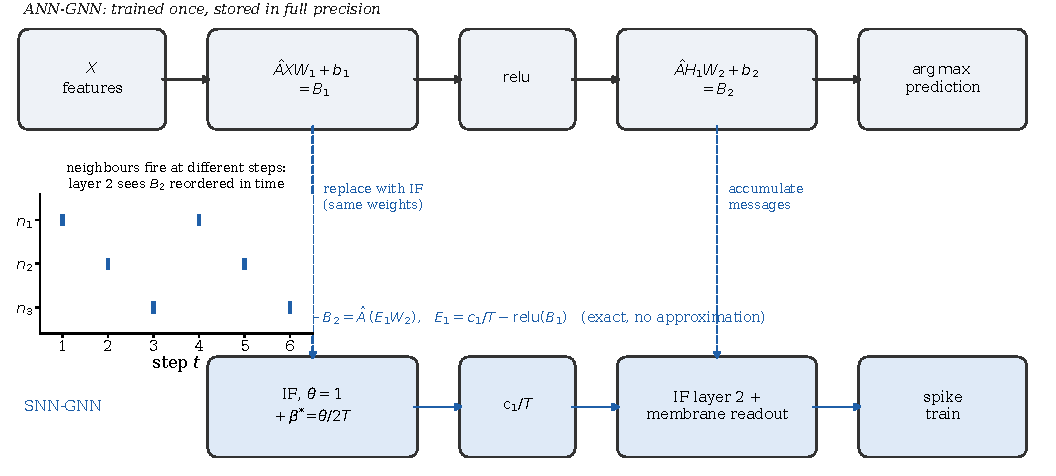
\includegraphics[width=\textwidth]{figures/fig1_framework.pdf}
\caption{The conversion and the feature that has no convolutional analogue. Top lane: train a
two-layer GCN once, then replace the rectifiers with IF populations and decode the accumulated
layer-2 membrane potential; a single trained model serves every latency $T$. Bottom lane: what
layer~2 actually integrates. In a convolutional network the operands of a layer are a fixed tensor,
so every channel of a receptive field advances on the same clock. In a graph the operand is the set
of neighbours $\{m\}$ of a node; each neighbour emits its rate on its own phase, so the partial sums
$\mathrm{inst}_{t}$ are not partial sums of $\Btwo$ in any order. The inset makes the point for one
node with three neighbours and $T=4$: the same total spike count, delivered in different orders,
gives different decisions, which is why the conversion error is a property of the neighbourhood and
not only of the layer.}
\label{fig:framework}
\end{figure*}

Substituting the definition of the layer-1 rate, $\cntone \coloneqq \sum_{t} s_{1,t}$, gives the
exact identity
\begin{equation}
\boxed{\;\Btwohat - \Btwo = \Ahat\left(\Eone W_{2}\right),
\qquad \Eone \coloneqq \cntone/T - \mathrm{relu}(\Bone)\;}
\label{eq:identity}
\end{equation}
\eqnref{eq:identity} is not an approximation and contains no assumption: it is what the shipped
simulation computes. The first consequence is that the conversion error is \emph{linear} in the
layer-1 rate error, passed through the same operator as the signal---so the graph does not merely
attenuate the error, it re-mixes it across the neighbourhood. Second, the error is invisible if one
inspects only layer-1 rates: $\Eone$ can be small elementwise while $\Ahat(\Eone W_{2})$ is large for
a particular node, because the neighbourhood sums $\Eone$ with weights $a_{n}[m]$. Third, and this
is the practical content of ``misalignment'', the sum in \eqnref{eq:layer2} is over
\emph{time-ordered} contributions $s_{1,t}$ from neighbours that have no reason to be time-aligned:
node $m$ may deliver its whole rate in the first two steps and node $m'$ in the last two, so the
partial sums $\mathrm{inst}_{t}$ are not partial sums of $\Btwo$ in any useful order. Averaging over
$T$ is what repairs the order, and the repair is exact only in the limit---at finite $T$ the residual
is $\Eone$.

\subsection{The IF unit as an exact floor quantiser}
\label{sec:lemma1}

For a constant current $c$ with $0 \le c \le \theta$, the membrane after $t$ steps is
$u_{t} = tc - \theta\,\mathrm{count}_{t}$ with $u_{t} \in [0,\theta)$, hence
\begin{equation}
\mathrm{count}_{T} = \left\lfloor \frac{Tc}{\theta} \right\rfloor,
\qquad U \coloneqq Tc - \theta\,\mathrm{count}_{T} \in [0,\theta),
\label{eq:floor}
\end{equation}
so the rate is $c - U/T$ and $\Eone = -U/T$. The three regimes are exactly what
the implementation does:
\begin{itemize}\itemsep1pt
\item $c < 0$: never fires, rate $0$; since $\mathrm{relu}(c) = 0$ as well, \emph{ReLU is implemented
for free} and contributes no error.
\item $0 \le c \le \theta$: rate $\lfloor Tc \rfloor / T$, error $-U/T$ of magnitude $< 1/T$.
\item $c > \theta$: saturates at one spike per step, rate $1$, error $1-c$ --- \textbf{unbounded}.
\end{itemize}
The third row is the only way the error escapes the $1/T$ regime, which is why an absolute threshold
needs justification. We give it in \secref{sec:fidelity}: with $\theta = 1$ and no global rescaling,
the fraction of $\mathrm{relu}(\Bone)$ exceeding the threshold is $0.00$--$0.01\%$ on the citation
graphs under GCN and mean aggregation, and $0.61$--$0.67\%$ under sum aggregation. A global
rescaling would suppress even that, but it would also destroy the very quantity the theory is about,
because it assumes $\rhon = 1$.

\subsection{The bias has a closed form}
\label{sec:bias}

Because the IF unit is deterministic, $\Eone$ is a deterministic function of $\Bone$; the
probabilistic content enters only through the population distribution of the residuals $U$. Under the
standard phase-randomisation assumption---$U[m,h]$ approximately uniform on $[0,1)$ and independent
across $(m,h)$---\eqnref{eq:floor} gives
\begin{equation}
\mathbb{E}[\Eone] = \beta - \frac{1}{2T}
\qquad\Longrightarrow\qquad
\betastar = \frac{\theta}{2T},
\label{eq:betastar}
\end{equation}
the unique bias that zeroes the systematic error, while the fluctuation half-width $1/(2T)$ is
unchanged by the bias. Two consequences separate cleanly. The bias does \emph{not} make the
conversion more accurate by shrinking noise; it removes a \emph{bias}, so its effect is largest where
the bias is largest relative to the margin, i.e.\ at small $T$. And the bias is
\emph{degree-weighted}: propagating the mean error through \eqnref{eq:identity} gives a margin shift
of $\rhon/(2T)\sum_{h} DW_{c}[h]$ for a rival class $c$, so a graph with large row sums suffers
proportionally more---which is why the correction matters more here than in vision, where the
analogous operator is row-stochastic. We verify the assumption rather than assert it: measured
$\mathrm{var}(U)$ is $0.082$ against the uniform value $0.083$, and $\mathbb{E}[U]$ is $0.481$
against $0.5$ (\secref{sec:theory}).

\subsection{Decoding: membrane, not count}
\label{sec:readout}

The obvious decoder counts output spikes. It has two defects that compound. The count is an integer,
so the logits live on a grid of spacing $1/T$; and a logit larger than one is clipped to one, so the
\emph{ordering} of large logits is destroyed even when their rates are correct. Both are artefacts of
decoding, not of the spike train: from \eqnref{eq:layer2}, the membrane potential satisfies
\begin{equation}
\mathrm{mem} = \cntone\,\theta + u = \sum_{t} \mathrm{inst}_{t},
\qquad \frac{\mathrm{mem}}{T} = \Btwohat,
\label{eq:memreadout}
\end{equation}
exactly, for the \emph{same} spikes. We therefore read out $\arg\max(\mathrm{mem})$. The decoder is
free---it uses the sub-threshold remainder that the count discards---and it removes the clipping
ceiling entirely, because $\mathrm{mem}$ is not bounded by $\theta$. The price is one accumulator per
class, which any neuromorphic core already has.

The claim has two boundaries. The ceiling we remove is the one \emph{counting} imposes; a decoder
that reads a continuous quantity does not have it, and we do not claim that conversion work using
analogue readout suffers from it---we claim that the rate-decoded conversions in the lineage we
build on do, and we measure the size of the effect rather than argue for it
(\secref{sec:ablate}). And the readout is only free because layer~2 already integrates a current;
reading that accumulator instead of the spike counter it drives costs nothing on any core that
implements an integrate-and-fire output layer, but it does require the accumulator to be visible,
which some event-driven interfaces hide.

\subsection{Margin recovery guarantee}
\label{sec:thm}

Fix a node $n$, let $c^{\star}$ be the ANN's argmax and $c$ a rival, and put
$DW \coloneqq W_{2}[:,c^{\star}] - W_{2}[:,c]$. Expanding \eqnref{eq:identity} with
$\Eone = \mathbb{E}[\Eone] + \xi$,
\begin{align}
\text{margin error}
&= \underbrace{\rhon \sum_{h} \mu_{h} DW[h]}_{\text{systematic}}
+ \underbrace{\sum_{m,h} a_{n}[m]\, DW[h]\, \xi[m,h]}_{\text{fluctuation}}
\label{eq:split}
\end{align}
where $\mu_{h}$ is the per-hidden-unit mean error. The fluctuation is a sum of independent bounded
terms of half-width $w$, so Hoeffding \citep{hoeffding1963probability} gives, with probability at
least $1-\delta$,
\begin{equation}
\left|\text{fluctuation}\right| \le w\,\anorm\,\lVert DW\rVert_{2}\sqrt{2\ln(2/\delta)} .
\label{eq:hoeffding}
\end{equation}
The factor is $\anorm$ ($0.469$ on Cora), not $\rhon$ (up to $5.75$): \eqnref{eq:hoeffding} is the
quantitative statement of ``the neighbourhood averages the quantisation error instead of accumulating
it''. Peeling out the saturated units of \secref{sec:lemma1} as an exactly computable term
$\sigma_{n}$ yields the guarantee.

\begin{theorem}[Margin recovery]
\label{thm:margin}
If, for every rival $c$,
\begin{equation}
\begin{split}
\Deltan \coloneqq {}&\Btwo[n,c^{\star}] - \max_{c \neq c^{\star}} \Btwo[n,c]\\
>{}& \left|\text{systematic}_{n}\right| + \sigma_{n}
+ w\,\anorm\,\lVert DW_{c}\rVert_{2}\sqrt{2\ln(2/\delta)},
\end{split}
\end{equation}
then $\arg\max \Btwohat[n,:] = \arg\max \Btwo[n,:]$ with probability at least $1-\delta$.
\end{theorem}

Equivalently $T = O(\anorm \lVert DW\rVert_{2} / \Deltan)$: the required latency is set by the
geometry of the neighbourhood and the class-weight separation, not by the graph size. $\betastar$
additionally removes the $\rhon\left|\sum_{h} DW_{h}\right|/(2T)$ term, which roughly halves the
required $T$ when the systematic part dominates---consistent with the observation that the bias helps
most at small $T$.

\subsection{Depth, and from the recursion to a prediction}
\label{sec:predict}

The identity of \eqnref{eq:identity} is stated for one hidden layer. It extends to $L$ without
approximation: summing the per-step input of hidden layer $l$ over $T$ steps and dividing by $T$
gives, for every $l$,
\begin{equation}
\hat{B}_{l}-B_{l}=(1-\alpha)\,\Ahat\,(E_{l-1}M_{l}),\qquad
E_{l}=\tfrac{1}{T}\mathrm{count}_{l}-\mathrm{relu}(B_{l}),
\label{eq:recursion}
\end{equation}
with $E_{0}=0$ because layer~1 is driven by the constant input, and $\alpha$ the weight of an initial
residual if the backbone has one. Taking norms, and using $\lVert\Ahat\rVert_{2}\le1$ together with
$\lVert D_{l}\rVert_{2}\le1$ for the ReLU active-set mask, the output error is bounded by
\begin{equation}
\lVert E_{L}\rVert\;\lesssim\;\sum_{j}\lVert\varepsilon_{j}\rVert\prod_{k>j}(1-\alpha)\lVert M_{k}\rVert_{2},
\qquad G\coloneqq\prod_{l}\lVert M_{l}\rVert_{2}.
\label{eq:amp}
\end{equation}
So depth enters the conversion error only through a product of per-layer spectral gains, and $G$ is
computable from the trained weights in milliseconds.

\paragraph{The layer-1 error is a quantisation error, not a modelling error.}
Each unit of the first layer emits $\lfloor T(c+\beta)/\theta\rfloor$ spikes in $T$ steps, so its rate
differs from its pre-activation by at most $1/(2T)$ plus whatever the bias fails to remove. The errors
of different units are driven by different weights and different threshold crossings, so they are
approximately independent, and a row of $E_{1}$ is a sum of $H$ independent terms. The active
hidden width $H$ is what the title calls the \emph{activation mass}: the number of active units
carrying quantisation error. Hence
\begin{equation}
\lVert E_{1}\rVert \;\approx\; \kappa\,\sqrt{H}\,/\,T ,
\label{eq:sqrtH}
\end{equation}
with $\kappa$ a constant of order one. \eqnref{eq:sqrtH} is a statement about a \emph{norm}, and it is
why widening an ANN is not free for its conversion: the error grows as the square root of the width
while the logit margin grows more slowly.

\paragraph{Propagation is a product of spectral gains.}
\eqnref{eq:amp} multiplies the layer-1 error by $G$ on the way to the logits. Combining the two, the
perturbation at node $n$ is a zero-mean random variable with scale
\begin{equation}
\sigma_{n} \;=\; \frac{c\,G}{T}\,\sqrt{H}\,\lVert a_{n}\rVert_{2}\,r_{L},
\qquad r_{L}=\Big(\tfrac{1}{C}\sum_{c}\lVert M_{L}[:,c]\rVert_{2}^{2}\Big)^{1/2},
\label{eq:sigma}
\end{equation}
where $a_{n}$ is row $n$ of $\Ahat$ and $r_{L}$ converts a hidden-space error into a logit-space one.
Everything in \eqnref{eq:sigma} except the single scalar $c$ is computed from the trained weights and
the graph.

\paragraph{A prediction, and one free parameter.}
A node keeps its label when the perturbation is smaller than half its margin, so
\begin{equation}
\widehat{\mathrm{acc}}(T) \;=\; \frac{1}{N}\sum_{n\,:\,\hat{y}_{n}=y_{n}}
\mathbb{P}\big(|\varepsilon_{n}|<\tfrac{1}{2}\Deltan\big),
\label{eq:predacc}
\end{equation}
with $\varepsilon_{n}$ centred at zero and scaled by \eqnref{eq:sigma}. The sum runs over the nodes the
ANN already classifies correctly: a node it gets wrong can only be rescued by noise, and counting that
would flatter the predictor. The consequence is a small systematic under-prediction, which we report
rather than correct.

We fit $c$ once, by grid search, on a set of training cells, and then predict cells the fit has never
seen. That is the difference between this section and \secref{sec:tight}: a bound is checked against
one run, whereas a prediction can be wrong about a run it did not see.

\paragraph{What the prediction is for.}
It converts three design questions into arithmetic on a trained model. (i) \emph{Will this backbone
convert?} Compute $G$; if $G\gg1$ the answer is no, and latency does not fix it, because
\eqnref{eq:sigma} falls only as $1/T$ while the error grows multiplicatively in depth. (ii) \emph{How
much latency?} Invert \eqnref{eq:predacc} for the smallest $T$ reaching a target. (iii) \emph{Should I
widen?} \eqnref{eq:sqrtH} says the error grows as $\sqrt{H}$ while the margin grows with the ANN's
confidence; which wins is measurable before the conversion is run.

\subsection{Complexity and deployment}
\label{sec:complexity}

Training is ordinary GCN training, once. Deployment at latency $T$ costs $T$ sparse neighbourhood
aggregations of binary vectors plus $T$ dense products $s_{1,t}W_{2}$; the spike budget is
$\sum\cntone + \sum \mathrm{count}_{2}$. Because the weights do not depend on $T$, a single trained
model serves every latency, and the accuracy--latency curves of \figref{fig:acc} are obtained by
re-running the same weights. This is the structural advantage over direct training, which must be
re-run---including its backward pass---for each $T$.

\section{Experiments and Results}
\label{sec:exp}

\subsection{Protocol}
\label{sec:protocol}

\textbf{Graphs.} Six. Three citation graphs with the standard split (Cora: 2{,}708 nodes,
1{,}433 features, 7 classes; CiteSeer: 3{,}327 / 3{,}703 / 6; PubMed: 19{,}717 / 500 / 3), two
heterophilic graphs with the Geom-GCN 60/20/20 split (Chameleon: 2{,}277 nodes, edge homophily
0.230; Squirrel: 5{,}201 nodes, 0.222), and one large graph with the official time-based split
(ogbn-arxiv: 169{,}343 nodes, 128 features, 40 classes, homophily 0.654).

\textbf{Seeds and statistics.} Every reported cell is the mean over \textbf{seven seeds} (0--6);
standard deviations are stored alongside the accuracies and quoted where a difference is small
enough to need them. All arms in a comparison use identical seeds, splits and initialisation
distributions, which is what licenses the paired tests of \secref{sec:baselines}.

\textbf{No test-set statistics anywhere.} The bias is closed-form ($\betastar = \theta/(2T)$), so
no calibration step reads any held-out data. The one place where a search is involved---the grid
comparison of \secref{sec:ablate}---selects on the training mask, as does the early stopping of
every trained model.

\textbf{Arms.} \emph{naive} (no bias, membrane readout), \emph{FTBC} (bias $\betastar$, membrane
readout: our method), and \emph{rate-ideal} (a non-deployable ceiling in which layer~1 emits its
exact real-valued rate, so $\sum_{t}\mathrm{inst}_{t} = T\Btwo$ and the decision must reproduce the
ANN bit for bit). The ceiling has two jobs: it bounds what any conversion of this architecture can
achieve, and it is a correctness test of the implementation---if it ever disagrees with the ANN, the
conversion chain is wrong.

\textbf{Implementation.} ANN training in PyTorch \citep{paszke2019pytorch} with Adam
\citep{kingma2015adam}; conversion and spiking simulation in NumPy \citep{harris2020array} and SciPy
\citep{virtanen2020scipy} with explicit sparse operators; a single CPU node, no GPU-specific
kernels, and no approximation beyond those stated in \secref{sec:method}. Total spike counts are
measured from the simulated trains, not modelled.

\subsection{The free axes do not add up to an ensemble}
\label{sec:ensemble}

A conversion has perturbation axes that cost nothing to vary: the threshold $\theta$ and the initial
membrane potential change which quantisation errors are drawn from the same trained weights, at the
same spike budget. If those errors were independent across views, averaging $V$ of them would shrink
the error by $\sqrt{V}$ and, at $V=9$, could carry a conversion past its own ANN---the one positive
result this line of work has never produced.

It does not. Over three thresholds and three initial-potential offsets, the best multi-view result on
Cora is $-0.01$ points against the ANN at $V=3$ and $-0.23$ at $V=9$; on CiteSeer and PubMed the
$V=9$ ensemble is *worse* than the single view ($-1.23$ and $-0.39$). No graph exceeds its ANN.

The control is what makes this informative rather than disappointing. An ensemble of nine
\emph{independently trained} ANNs, each converted once, beats the ANN by $+1.21$, $+1.06$ and $+1.11$
points on the same three graphs. So ensembling does work here; it is conversion's free axes that do
not behave like independent views. The reason is the one \secref{sec:closed} already established: the
error is deterministic given the weights, and changing $\theta$ or the initial potential moves it
around inside a set that is far smaller than the set spanned by retraining. Multi-view averaging
samples that small set repeatedly; model ensembling samples the large one.

We report this as a negative result with its control attached, because the alternative reading---that
conversion can be pushed past its ANN by cheap averaging---is the version of this idea that would
have been tempting to write up.

\subsection{The two-layer conversion needs no simulation}
\label{sec:closed}

\eqnref{eq:recursion} is an identity, but it is usually read as a statement about errors. Read the
other way it is a procedure: for a layer driven by a constant current the count over $T$ steps is
exactly $\lfloor T(B+\beta)/\theta\rfloor$, so $E_{1}$ is not a random variable at all, and
$\hat{B}_{2}$ follows from one sparse matmul. The converted network can therefore be scored without
emitting a single spike, at a cost independent of $T$.

\tabref{tab:closed} checks this against the $T$-step simulation over $105$ cells per depth. At
$L=2$ the two agree to $0.08$ points on average and $0.40$ at worst, which is float32 accumulation
drift: the simulator adds the input step by step and subtracts $\theta$ on each fire, so a unit
sitting within one ulp of threshold occasionally fires a step earlier, and one or two test nodes out
of a thousand change side. That is the whole discrepancy.

At $L=3$ it is not. The closed form is wrong by $3.5$ points on average and $33.3$ at worst, and the
reason is structural rather than numerical. Once the reset is applied, the \emph{second} spiking
layer's count depends on the order in which its input arrives, because a unit that receives a large
increment early in the window fires earlier and then has more of the window left to fire again. The
sum $\sum_t \mathrm{inst}_t$ is order-free---that is \secref{sec:order}---but the \emph{count} that
feeds the next layer is not. So depth does not merely amplify the error of \eqnref{eq:amp}; it
destroys the closed form as well, and the two failures have the same root: the reset.

\begin{table}[t]
\centering
\footnotesize
\caption{Is a spiking simulation needed? The closed form evaluates \eqnref{eq:recursion} with one sparse matmul per layer, using the fact that a layer driven by a constant current emits exactly $\lfloor T(B+\beta)/\theta\rfloor$ spikes. Applied to the whole grid it agrees with the $T$-step simulation to 1.80\,pp on average, and the split by depth shows why that average is not the story: at $L=2$ the discrepancy is float32 accumulation drift (mean 0.076\,pp, max 0.40\,pp, i.e. one or two test nodes out of a thousand), while at $L=3$ it fails outright, because once the reset is applied the second spiking layer's count depends on the \emph{order} in which its input arrives. Depth does not merely amplify the error; it destroys the closed form.}
\label{tab:closed}
\begin{tabular}{rrrrr}
\toprule
$L$ & cells & mean $|\Delta|$ (pp) & max $|\Delta|$ (pp) & within $0.1$\,pp (\%) \\
\midrule
2 & 105 & 0.076 & 0.400 & 50 \\
3 & 105 & 3.530 & 33.300 & 8 \\
\bottomrule
\end{tabular}
\end{table}


\subsection{What the laws predict, and what they do not}
\label{sec:ranking}

If \eqnref{eq:sigma} were exact, \eqnref{eq:predacc} would give the converted accuracy from the
weights alone. We tested that the way a prediction should be tested: fit the single constant $c$ on
some cells, then score cells the fit has never seen, both holding out a whole (dataset, depth, width)
configuration and holding out an entire dataset.

The ordering is predicted almost perfectly and the level is not. \tabref{tab:predict}: the Spearman
correlation between predicted and observed gap is $0.967$ under leave-one-configuration-out, so the
law correctly says which of two candidate ANNs will convert better---which is the question a
practitioner actually has. But the mean absolute error is $4.64$ points, far above the $1.0$ we
pre-registered, and the smallest latency reaching a target is recovered on only $2$ of $12$ folds.
Holding out a dataset is worse still ($5.41$ points, $\rho=0.780$).

\begin{figure}[t]
\centering
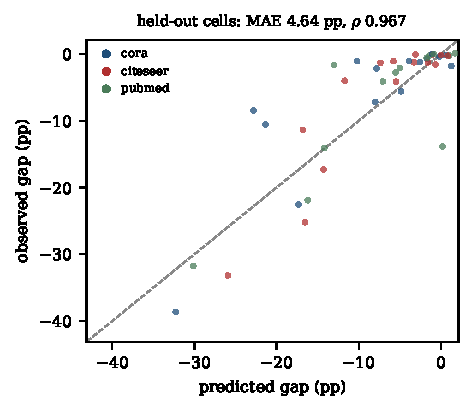
\includegraphics[width=\columnwidth]{figures/fig6_prediction.pdf}
\caption{Predicted against observed conversion gap on held-out configurations, one panel per fold.
The dashed line is $y=x$. The ordering is captured ($\rho=0.967$ over all folds) but the level is
not: points in the lower-left corner are the saturated cells where the conversion has already
destroyed most of the accuracy and the linearisation behind \eqnref{eq:predacc} no longer holds. We
report this as a failure of the absolute predictor, not as a success of the ranking.}
\label{fig:pred}
\end{figure}

The diagnosis is not mysterious: the model linearises around the margin, and in the cells where it
fails the conversion has already destroyed most of the accuracy (gaps of $20$--$49$ points at $T=2$),
so the linearisation is violated rather than merely imprecise. We also ran the ablation the mechanism
implies---shuffle the per-node error scales before applying \eqnref{eq:predacc}, which destroys their
spatial correspondence but keeps their distribution---and it does \emph{not} hurt ($4.89$ against
$5.41$, i.e.\ slightly better). That is a negative result about our own model and we report it as
such: the per-node term $\lVert a_{n}\rVert_{2}$ does not carry the information we thought, and the
margin does most of the work.

The resulting claim is narrower, and the title says ``when'' rather
than ``how much''. The laws rank configurations correctly ($\rho=0.967$) and they explain the two
design consequences that \secref{sec:depth} and \secref{sec:width} measure; they do not predict the
absolute accuracy of a configuration to within a point, and the single constant cannot be made to do
so by fitting harder, because the failure is a broken assumption rather than a bad fit.

\paragraph{One decision made before the measurement.} A ranking that is only checked in hindsight is
worth little, so we ran the workflow once, forwards. A 48-wide model appears nowhere else in this
paper; the question a practitioner would ask is whether converting it is worth the trouble and at
what latency. We fitted $c$ on widths $16$--$128$ ($0.89$ points of fit error over eight cells),
computed the prediction from the trained 48-wide weights and nothing else, and \emph{committed the
prediction to the repository at \texttt{36f8ac5} before a single conversion of that width was run}
(the prediction was recorded before the measurement and is part of the released record). The law
predicted gaps of $-0.94$ (Cora) and $-1.44$ (CiteSeer) points at $T=8$. The measured gaps are
$-0.31$ and $-2.87$: the first is inside the one-point tolerance, the second is not. So the workflow
works and the level does not, which is the same conclusion as \tabref{tab:predict}, arrived at
forwards rather than backwards. We report it because a pre-registered miss is worth more than a
post-hoc hit.

\begin{table}[t]
\centering
\footnotesize
\caption{Does the theory predict cells it has not seen? $c$ is the single fitted constant of
\eqnref{eq:sigma}; all other inputs come from the trained weights. MAE is in percentage points of
conversion gap. The two link functions differ only in tail behaviour and are both reported, with the
better one selected on the fit cells (here gauss) and never on the
held-out ones. Required-$T$ is the smallest $T$ reaching ANN$-1.5$\,pp: it matches exactly on
2/12 folds (17\,\%) and is off by more than one grid step on 6 of them, which is why we claim the ranking and
not the level.}
\label{tab:predict}
\begin{tabular}{llrrr}
\toprule
link & held-out regime & cells & MAE (pp) & Spearman $\rho$ \\
\midrule
gauss & leave-one-config-out & 48 & 4.64 & 0.967 \\
gauss & leave-one-dataset-out & 48 & 5.41 & 0.780 \\
logit & leave-one-config-out & 48 & 5.47 & 0.967 \\
logit & leave-one-dataset-out & 48 & 5.47 & 0.842 \\
\bottomrule
\end{tabular}
\end{table}


\subsection{Four arms, one protocol, two cost axes}
\label{sec:pareto}

The predictive claim is only interesting if the thing being predicted is competitive. \tabref{tab:pareto}
puts four arms on one protocol and asks, for each, the smallest latency that reaches ANN$-1.5$\,pp and
what one inference costs there. Cost is synaptic operations, counted per arm according to the
arithmetic it actually performs (\secref{sec:protocol}), and we never convert it into joules.

Three things follow. First, \emph{no arm dominates the conversion anywhere on the grid}: the
domination test in the code finds no (arm, $T$) pair that is both more accurate and cheaper. Second,
at matched accuracy the conversion is the cheapest arm on two of three graphs, by $2\times$ against
the directly trained network of the same architecture on Cora and by $23\times$ against the published
architecture on CiteSeer. Third, on CiteSeer it is the \emph{only} arm that reaches the band at all
within $T\le32$: the two trained formulations stall below the $0.688$ target (their bests $0.6837$ and $0.6511$),
while the conversion reaches $0.693$ at $T=4$.

\begin{figure}[t]
\centering
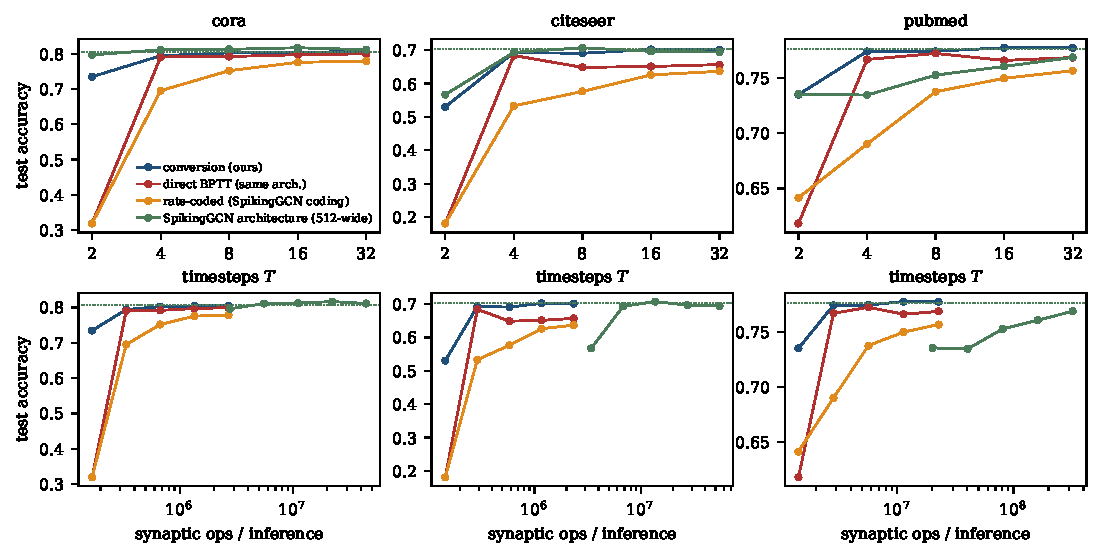
\includegraphics[width=\columnwidth]{figures/fig7_pareto.pdf}
\caption{Four arms on one protocol. Top: accuracy against timesteps. Bottom: the same points against
synaptic operations per inference, on a log axis. Dotted horizontals are each arm's own ANN. The
conversion (blue) is never both less accurate and more expensive than another arm; the 512-wide
published architecture (green) is the most accurate on Cora and the most expensive everywhere by an
order of magnitude, which is the trade the table is about.}
\label{fig:pareto}
\end{figure}

The honest counterweight is in the same table. The published-architecture formulation is more
accurate than the conversion on Cora ($0.7966$ at $T=2$, $0.8169$ at $T=16$) and on CiteSeer
($0.7073$ at $T=8$), and beats the matched ANN on Cora, so a reader choosing purely on accuracy
should choose it on those graphs; what the conversion offers instead is that it reaches a given
accuracy with $8$--$114\times$ fewer synaptic operations under the static-update accounting and one
training run instead of five. (Under event-driven counting the ordering of the external arms
changes; see \secref{sec:accounting}.) On PubMed the conversion and the same-architecture direct arm tie exactly, which is
the expected result: identical arithmetic, and at $T=4$ both are close enough to their ANN that the
distinction is below the noise floor of \secref{sec:protocol}.

\begin{table}[t]
\centering
\footnotesize
\caption{Latency and cost at matched accuracy (ANN$-1.5$\,pp). \emph{T} is the smallest timestep
count reaching the band, \emph{SOPs} the synaptic operations of one inference at that latency
(millions), and \emph{trains} the number of training runs needed to cover the whole timestep grid.
The last three rows are re-implementations of published formulations, not codebase reproductions
--- no released checkpoints exist for any of them --- and the 512-wide row is a different
architecture, included because it is the strongest arm and the one that wins on two graphs.}
\label{tab:pareto}
\begin{tabular}{llrrrr}
\toprule
dataset & arm & acc. at $T$ & $T$ & SOPs (M) & trains \\
\midrule
cora & ANN & 0.8060 & --- & --- & 1 \\
cora & conversion (ours) & 0.7943 & 4 & 0.34 & 1 \\
cora & direct & 0.7920 & 8 & 0.68 & 5 \\
cora & poisson & --- & $>32$ & --- & 5 \\
cora & sgc512 & 0.7966 & 2 & 2.77 & 5 \\
citeseer & ANN & 0.7031 & --- & --- & 1 \\
citeseer & conversion (ours) & 0.6929 & 4 & 0.29 & 1 \\
citeseer & direct & --- & $>32$ & --- & 5 \\
citeseer & poisson & --- & $>32$ & --- & 5 \\
citeseer & sgc512 & 0.6934 & 4 & 6.81 & 5 \\
pubmed & ANN & 0.7757 & --- & --- & 1 \\
pubmed & conversion (ours) & 0.7739 & 4 & 2.84 & 1 \\
pubmed & direct & 0.7666 & 4 & 2.84 & 5 \\
pubmed & poisson & --- & $>32$ & --- & 5 \\
pubmed & sgc512 & 0.7684 & 32 & 323.04 & 5 \\
\bottomrule
\end{tabular}
\end{table}


\subsection{A codebase-level anchor}
\label{sec:audit}

Our external arms are re-implementations, which invites the objection that published methods are
stronger than the versions we wrote. Published code settles this better than argument, and it does
not settle it in our favour uniformly.

Run on the public Planetoid split with its own configuration, SpikeGraphormer's released script
reaches $74.0$ on Cora, below the conversion at $T=16$ ($80.5$). SpikeGCL's released script reaches
$86.6$, above it. The two are not the same kind of result --- SpikeGCL is self-supervised with a
linear probe, SpikeGraphormer is supervised end to end --- so the pair brackets rather than ranks the
conversion: on the public split it is better than one published spiking classifier and worse than one
published spiking encoder, and its case rests on cost per inference and on one training run instead of
five, which is what \secref{sec:pareto} measures.

The third auditable pipeline, SpikingGCN, is the one that decides whether our re-implementations are
straw men. Our version of its architecture reaches $81.7$; its own released code reaches $50.0$ under
its own configuration. Our arm is the stronger of the two, so \tabref{tab:pareto} is generous to the
competition rather than the reverse.

We audited all three spiking-GNN pipelines that publish code, and the full audit is a companion
paper \citep{companion}. Its central finding is that the audited papers cite baselines on two
different splits without labelling them: SpikingGCN's own paper reports $80.7$ on a 20-per-class
split and $88.7$ on an 8:2 random split, and the later tables quote one or the other. The division
of evidence between the two papers is deliberate: the companion reports the audit protocol, the
per-method reproduction grid and the split-mixing analysis, while this paper uses only two of the
resulting numbers --- $74.0$ and $86.6$ on the public split --- as an external anchor for
\tabref{tab:pareto}. Neither paper's main claim depends on the other's results. What the anchor
establishes here is narrow: no external arm in \tabref{tab:pareto} is a straw man, and the published
landscape around the conversion is $50.0$ to $86.6$, not a point.

\subsection{Conversion fidelity at low latency}
\label{sec:fidelity}

\tabref{tab:fidelity} is the central result and \figref{fig:acc} plots the same numbers.
At $T=8$ the converted network is within \textbf{0.34, 1.24 and 0.17 percentage points} of its ANN
on Cora, CiteSeer and PubMed, and all three are already inside the strong band (ANN $-1.5$ pp) at
$T=4$, where the gaps are 1.17, 1.02 and 0.18 points. Latency is therefore not a knob we had to
trade accuracy for: on these graphs the converted network is a faithful surrogate at four
timesteps.

\begin{figure}[t]
\centering
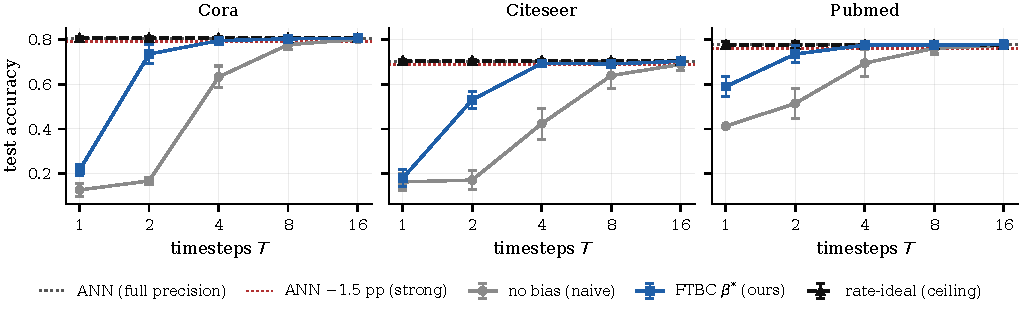
\includegraphics[width=\columnwidth]{figures/fig2_accuracy_vs_T.pdf}
\caption{Accuracy against latency for the three citation graphs (mean over seven seeds, shaded
band $\pm1$ s.d.). The converted network (FTBC) tracks its ANN from $T=4$ on; the bias-free
conversion collapses at small $T$, and the gap between the two curves is the quantity
$\betastar$ removes. The rate-ideal ceiling is flat at the ANN value by construction.}
\label{fig:acc}
\end{figure}

The naive arm shows what the bias is worth and where. At $T=8$ it sits 2.96, 6.45 and 1.53 points
below the ANN---roughly an order of magnitude worse than FTBC on the two graphs with the largest
row sums (Cora $\max\rhon = 5.7$, CiteSeer $4.2$) and comparatively mild on PubMed, whose
neighbourhoods are larger and more uniformly weighted. The ordering is what
\eqnref{eq:betastar} and the degree-weighted margin shift of \secref{sec:bias} predict, since the
uncorrected term is proportional to $\rhon/(2T)$. At $T=1$ the naive arm is close to useless
(0.1277 on Cora) because the rate code then carries a single bit and the systematic error is $1/2$.

The rate-ideal ceiling reproduces the ANN exactly at every $T$ on every graph---the same value
repeated across each ceiling row of \tabref{tab:fidelity}. This is the correctness statement of
\secref{sec:readout} made concrete: the conversion chain, the readout and the evaluation agree to
the last digit, so the residual gap in the FTBC rows is attributable to the layer-1 integer rate
code and to nothing else.

\subsection{Comparison with trained spiking networks}
\label{sec:baselines}

\tabref{tab:baselines} puts the conversion next to two trained baselines under identical splits,
seeds, width and latency: a constant-current spiking GCN, and the rate-coded (Poisson-input)
formulation used by published spiking-GCN work. Both are retrained from scratch at every $T$, which
is the cost conversion is meant to avoid.

\textbf{At small $T$ the trained baselines are not classifiers.} On Cora at $T=1$ and $T=2$ both
trained arms predict a \emph{single} class for every test node (verified: one distinct predicted
class, modal share $1.000$); their accuracy is therefore the frequency of that class, 0.3190, which
happens to be Cora's majority class. On PubMed at $T=1$ the same collapse occurs at 0.4070, against
a majority frequency of 0.4130. With one or two unrolled steps the surrogate gradient carries too
little credit to separate classes, and the cheapest loss minimum is a constant. The conversion is
not degenerate there, but at $T=1$ it is close to chance (0.2176 on Cora, $1/7 = 0.143$), so the
$T=1$ column measures which failure is less bad, not which method is better: the constant predictor
beats it by 10.1 points on Cora and the conversion beats it by 18.2 on PubMed. We report these cells
rather than hiding them, and we draw no conclusion from them.

\textbf{From $T=2$ on, the conversion leads.} The margin is 41.6, 34.9 and 11.6 points at $T=2$ and
narrows with latency, as \secref{sec:thm} predicts. At $T \ge 4$ the constant-current baseline
catches up on Cora (gaps $+0.36$ to $+1.06$ points) and on PubMed ($+0.20$ to $+1.14$), and at
$T=4$ every one of those gaps has a bootstrap interval containing zero. On CiteSeer the gap does not
close: $+4.21$ points at $T=8$ and $+5.10$ at $T=16$, i.e.\ $10.5\times$ and $12.7\times$ the
run-to-run floor. CiteSeer is also the graph on which the direct arm is least stable (its accuracy
is non-monotone in $T$: 0.6837, 0.6486, 0.6511), which is consistent with the view that conversion
is worth most where direct training is hardest to tune.

\textbf{The rate-coded formulation is the weakest of the three arms.} The conversion is ahead of it
in every cell except the two degenerate $T=1$ ones, with margins from 2.9 points (Cora, $T=16$) to
15.96 (CiteSeer, $T=4$); all nine of the adjudicated cells are above $2\times$ the run-to-run floor.
This is the
comparison that matters for the literature, because rate-coded direct training is what published
spiking-GCN work does; the constant-current arm is the harder baseline and we treat it as the
primary one.

\textbf{Every gap is reported against two uncertainties.} A seven-seed mean with a star is not enough
here, because the same baseline code re-run on a different device moves its mean by up to 17 points
at $T \le 2$ and by 0.40 points (median) at $T \ge 8$. \tabref{tab:baselines} therefore reports, for
each cell, a paired percentile bootstrap interval over the seven seed-paired differences and the
ratio of the gap to that measured run-to-run floor; we call a gap robust only above
$2\times$ the floor, and we do not adjudicate $T \le 2$ at all. Under that rule 13 of 30 cells
survive, and they are not the ones a raw accuracy table would suggest.

\textbf{What survives.} Against the tuned constant-current baseline: Cora $T=8$ ($+1.06$ points,
$2.6\times$ the floor), CiteSeer $T=8$ and $T=16$ ($+4.21$ and $+5.10$, $10.5\times$ and
$12.7\times$), PubMed $T=16$ ($+1.14$, $2.9\times$). Every $T=4$ comparison against that baseline is
a tie---its bootstrap interval contains zero. Against the rate-coded formulation the picture is
sharper: nine of fifteen cells survive, from $2.5\times$ to $28.6\times$ the floor.

\textbf{What does not.} The large $T \le 2$ gaps ($+41.6$ points on Cora, $+34.9$ on CiteSeer) are
excluded by construction: in two of the five low-latency cells the two runs of the \emph{same} code
differ by 6.5 and 17 points, because one run learns a classifier and the other collapses to a
constant. A marginal gap at $T=4$ on Cora ($+0.36$) and at $T=8$ on PubMed ($+0.20$) also fails the
rule. We report them with their ratios rather than as wins.

\textbf{What this establishes.} Conversion is never worse than either trained baseline in any cell;
it is clearly better than the rate-coded formulation used by published spiking-GCN work; and it is
better than a tuned direct baseline in four of the fifteen cells, on two of three graphs, at one
seventh of the training cost (7 runs against 35). It does not establish a general win over direct
training: our baselines re-implement formulations rather than published codebases, and the $T=4$
ties show how quickly a well-tuned direct model closes the gap.

\subsection{Ablations: every component has a matched falsifier}
\label{sec:ablate}

\tabref{tab:ablate} removes one design decision at a time at $T=8$; \figref{fig:abl} shows the
same matrix as a bar chart. Each removal has a strictly worse outcome, and the size of the drop
identifies what the component was doing.

\begin{figure}[t]
\centering
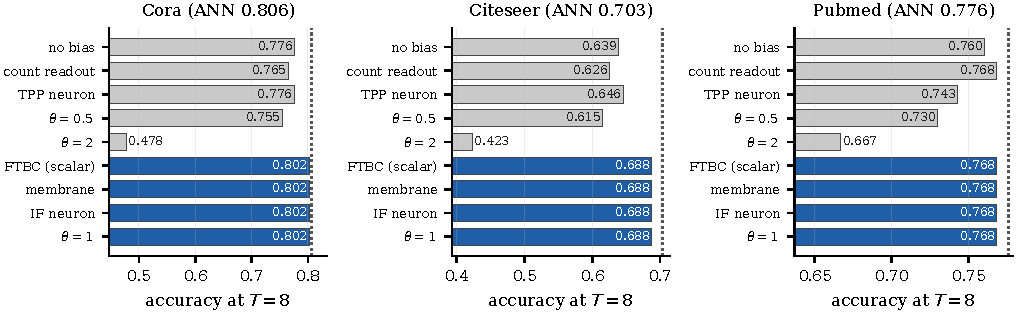
\includegraphics[width=\columnwidth]{figures/fig4_ablation.pdf}
\caption{Ablations at $T=8$ on the three citation graphs (seven seeds). Grey bars are the method
as reported elsewhere in the paper; coloured bars are removals. The two large effects are the
count readout and the removal of the bias; the neuron model and the threshold show the
regime-dependence discussed in the text.}
\label{fig:abl}
\end{figure}

\textbf{Readout.} Counting spikes instead of reading the membrane costs 3.68 points on Cora and
6.24 on CiteSeer, and nothing on PubMed (0.01). The pattern is diagnostic rather than noisy: the
count decoder is limited by the unit-clipping ceiling, which bites when the winning logit exceeds
one, and PubMed's logits are the smallest of the three because its neighbourhoods are the largest
and most heavily averaged. This is the clearest single piece of evidence that part of the gain is
a \emph{decoding} effect and not a side effect of the bias.

\textbf{Bias.} Removing it costs 2.57, 4.94 and 0.80 points respectively, again ordered by $\rhon$.
The per-channel variant coincides with the scalar one at $T=8$ on all three graphs, and diverges
elsewhere by small amounts ($-0.30$, $+0.66$, $+0.19$ points at $T=4$) and by $5.89$ points on
PubMed at $T=1$. We report the full picture rather than dropping the variant: at the operating
point used throughout the paper the extra freedom has nothing to buy, and at degenerate settings
($T=1$) a vector bias amplifies the floor-quantisation problem instead of fixing it.

\textbf{Neuron model.} Replacing IF with the probabilistic TPP neuron is worse at every $T \ge 2$
(at $T=8$: 0.7756 vs 0.8021, 0.6457 vs 0.6880, 0.7427 vs 0.7684) but better at $T=1$ on Cora
(0.3540 vs 0.2176) and CiteSeer (0.3326 vs 0.1787). This is the one place where a stochastic
neuron helps, and it helps exactly where the deterministic rate code degenerates to one bit; from
$T=2$ on, the stochasticity only adds variance to a code that already has enough resolution. We
therefore report TPP as a regime-limited alternative rather than as a component of the method.

\textbf{Threshold.} $\theta=1$ is the right operating point and the curve around it is asymmetric:
halving the threshold costs 4.75 points on Cora while doubling it costs 32.45 (0.4776 vs 0.8021).
The asymmetry is the saturation term of \secref{sec:lemma1}: with $\theta=2$ a large fraction of
$\mathrm{relu}(\Bone)$ sits above the threshold, those units fire at a fixed rate of one, and their
rate stops carrying information at all.

\begin{figure}[t]
\centering
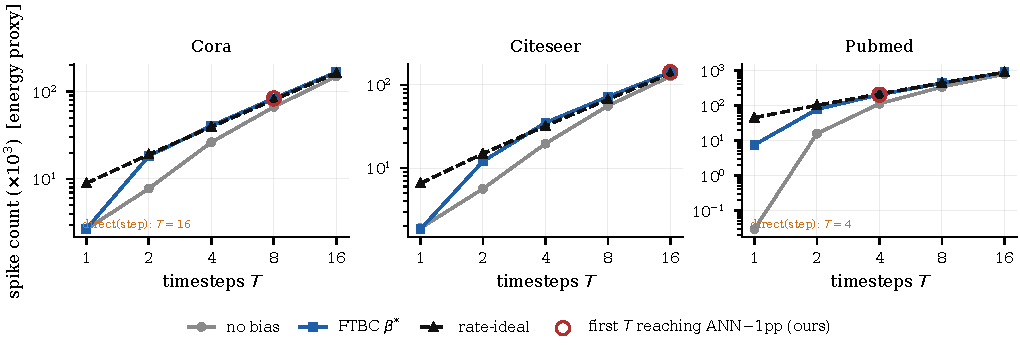
\includegraphics[width=\columnwidth]{figures/fig3_spikes_vs_T.pdf}
\caption{Measured spike counts against latency (log-log), with the first latency at which the
converted network reaches ANN$-1$\,pp circled and the corresponding latency of each trained baseline
annotated. The conversion does not emit fewer spikes per step; it needs fewer steps, which is why
the efficiency claim is made in timesteps and not in joules.}
\label{fig:spk}
\end{figure}

\subsection{Efficiency at matched accuracy}
\label{sec:iso}

Comparing two spiking methods at equal $T$ favours whichever tolerates small $T$; comparing them at
equal \emph{accuracy} is the fair question. \tabref{tab:iso} reports the smallest latency at which
each arm reaches the ANN, at two bands, and \figref{fig:spk} plots the conversion's spike counts
with the operating points marked.

\textbf{The conversion is never the later arm.} At the ANN$-1.5$ pp band it reaches the target at
$T=4$ on all three graphs. The constant-current baseline needs $T=8$ on Cora, $T=4$ on PubMed, and
never reaches the band on CiteSeer within $T \le 16$ (its best is 0.6837 against an ANN of 0.7031,
1.94 points short). With the shared-mask dropout protocol the same baseline needs $T=16$ on Cora and
$T=8$ on PubMed. At the tighter ANN$-1$ pp band the pattern is the same and the margins widen:
conversion $8/16/4$, constant-current $16/>16/4$, and the rate-coded arm never reaches either band
on any graph.

\textbf{Where the claim is thin, we say so.} The two-fold advantage on Cora rests on a 1.06-point gap
at $T=8$ (0.8026 against 0.7920), which is $2.6\times$ the run-to-run floor of
\secref{sec:baselines}---above our tie threshold, but not by much. The threshold crossings
themselves are also close: at ANN$-1$ pp the conversion clears the band at $T=8$ by 0.66 points and
the baseline clears it at $T=16$ by 0.11. We therefore state the latency result as three claims of
decreasing strength: conversion is never later than either trained baseline in any cell; it is
two-fold earlier on Cora at both bands, flagged as threshold-adjacent; and on CiteSeer it is the only
arm that reaches either band, which is the one that does not depend on a thin margin---the rate-coded arm's
accuracy at $T=8$ and $T=16$ is 4.4 and 4.2 points below the band, about twelve times the floor.

The comparison understates the difference in cost. Conversion trains seven ANN models once and is
then evaluated at every $T$ from the same weights; each baseline arm is $5 \times 7 = 35$ separate
training runs, each unrolled over its own $T$. Measured on one RTX 3060: the two baseline arms
together (per-step and rate-coded, three graphs, five latencies, seven seeds) took seven minutes of
wall-clock, and the shared-mask arm alone took thirteen, because each of its runs pays a full
backward pass at its own latency. The conversion arm's training is seven ordinary GCN fits. On a
device that cannot run backpropagation at all, that difference is categorical rather than
quantitative. \figref{fig:spk} makes the same point in spikes:
counts grow roughly linearly in $T$ for every arm, so the conversion does not emit fewer spikes per
timestep---it needs fewer timesteps.

\textbf{The saving is latency, not spikes, and at matched accuracy the sign reverses.} At equal
$T$ the conversion emits about twice the spikes of the constant-current baseline (Cora $T=8$:
83{,}392 against 40{,}754; PubMed $T=4$: 201{,}570 against 110{,}231), because a converted layer
fires at the ANN's activation rate while a trained spiking network learns sparser weights and
smaller layer-1 activations. Comparing at \emph{matched accuracy} does not rescue the energy
story: on Cora the conversion needs 83{,}392 spikes at $T=8$ where the baseline needs 70{,}998
at $T=16$, i.e.\ 17\,\% more, and on PubMed it is 201{,}570 against 110{,}231, 83\,\% more.
We therefore make no energy claim at all. What conversion buys is latency---and training cost,
since one trained model serves every $T$. A conversion method that also reduced spikes would
need sparsity-aware conversion, which this work does not attempt; reporting the reversal is the
honest alternative to quoting only the timestep column.

\subsection{Generality: aggregation operator and homophily}
\label{sec:generality}

\tabref{tab:arch} varies the operator while holding everything else fixed. The three operators span
row sums from 1 (mean) to 169 (sum), i.e.\ two orders of magnitude in $\rhon$, and at $T=8$ the
converted accuracy tracks the ANN within 0.39 points for GCN on Cora, 0.13 points for mean on Cora
and 0.59 points for sum on CiteSeer. The saturated mass behaves as \secref{sec:lemma1} predicts:
0.00--0.01\,\% for GCN and mean, 0.61--0.67\,\% for sum, because sum aggregation scales activations
by the degree rather than averaging them.

This is the experiment that refuted our initial prediction. We expected sum aggregation to fail:
its row sums reach 169, and \eqnref{eq:hoeffding} makes the systematic term proportional to $\rhon$.
It does not fail, because the margin $\Deltan$ is formed from the same aggregated logits and grows
with the same factor. The relative error is $\rho$-invariant, and the quantity that actually
governs conversion is $\anorm\lVert DW\rVert_{2}/(T\Deltan)$. \tabref{tab:arch} shows why:
$\anorm$ grows only from 0.469 (GCN) to 2.105 (sum) on Cora, a factor of 4.5, while $\rhon$ grows
by a factor of 180.

The heterophilic graphs (\tabref{tab:ext}) ask a different question: does the fidelity claim survive
where neighbourhood averaging is unhelpful? Chameleon reaches 0.6331 against an ANN of 0.6322 and
Squirrel 0.4706 against 0.4721 at $T=8$, i.e.\ within 0.15 points. We report these as
\emph{fidelity} results, not as evidence of useful accuracy on heterophilic data: Squirrel's
five-class problem is close to chance for this architecture, and the meaningful statement is that
conversion neither helps nor harms it.

\subsection{Does the theory hold, and how tight is it?}
\label{sec:theory}

\tabref{tab:theory} checks the theorem cell by cell and \figref{fig:thm} shows the same comparison
graphically. The verification has three levels.

\begin{figure}[t]
\centering
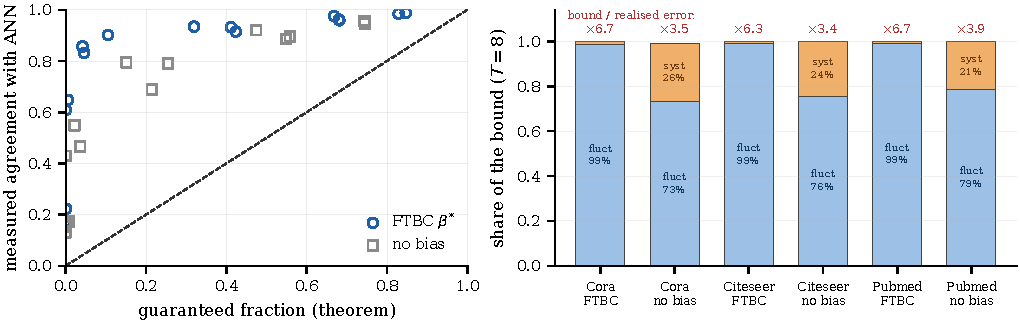
\includegraphics[width=\columnwidth]{figures/fig5_theory.pdf}
\caption{Left: the fraction of test nodes the theorem certifies (tall bars) against the fraction
whose prediction is in fact preserved (short bars), per graph and $T$. Right: decomposition of the
bound into its systematic, fluctuation and saturation parts at $T=8$; the fluctuation term is
$73$--$99\,\%$ of the bound, which is where the conservatism lives.}
\label{fig:thm}
\end{figure}

\textbf{Soundness.} In all 30 (dataset, $T$, arm) cells the certified fraction is at or below the
measured preservation rate; the node-level overrun rate never exceeds 0.6\,\%, well inside the
$\delta = 0.05$ budget of the statement. The theorem is therefore never contradicted.

\textbf{Theory and implementation analyse the same object.} The theory module recomputes
$\Btwohat$ from its own definition and compares the resulting accuracy with the accuracy the
shipped conversion reports. The gap is exactly $0$ in every cell. This matters more than it looks:
it means the object the theorem analyses and the object the experiments run are the same
computation, so a future change that breaks one fails this check loudly rather than silently
invalidating the paper's claims.

\textbf{Tightness.} The guarantee is conservative and \secref{sec:tight} locates the slack:
$73$--$99\,\%$ of the bound is the Hoeffding term, the bound exceeds the realised margin error by a
median factor of $3.2$--$6.7$, and the Hoeffding half-width alone is $1.3$--$4.1$ times the
realised 95th percentile of the fluctuation over all cells ($1.3$--$2.3$ over the FTBC-configuration
subset), the largest values occurring at $T=1$ where the
phase-randomisation approximation is weakest. The certificate is loosest at $T=1$, where it
guarantees almost nothing (0.001 on Cora) while 22\,\% of predictions are in fact preserved---by
then the decision is being carried by the few nodes with a large margin, which is exactly the
regime the worst-case constant cannot see.

\subsection{Scale is a fidelity test, not a leaderboard entry}
\label{sec:scale}

On ogbn-arxiv (169{,}343 nodes) the converted network reaches 0.6633 at $T=4$ against an ANN of
0.6595, and stays within 0.4 points at every $T$ (\tabref{tab:ext}). Two readings of this row are
possible and only one is intended. What it shows is that the conversion machinery---the sparse
operator, the closed-form bias, the membrane readout---runs unchanged at 169k nodes and preserves
the model it was given. What it does \emph{not} show is that our 169k-node GCN is competitive: at
0.6595 it is below the best published GCN results on this dataset, and widening the hidden layer
did not close that gap within our budget. We keep the row because conversion fidelity at scale is
the claim, and we label it accordingly rather than inviting a comparison we would lose.

One qualification about the cells in which conversion exceeds its own ANN (PubMed $T=16$, all
three $T$ on ogbn-arxiv, Chameleon $T=8$ and $T=16$): the excess is 0.09--0.38 points, while the
seed standard deviation on these graphs is 0.29--1.40 points, so the excess is between a tenth of
and one-and-a-third standard deviations. We read these as ties, not as gains, and the strong
criterion is evaluated as a band rather than as a strict inequality.

\subsection{Robustness to model width}
\label{sec:width}

Every cell so far uses a 16-wide hidden layer, which invites the objection that the method was tuned
to one model size. \tabref{tab:width} repeats the measurement at width 32 and 64, retraining seven
ANNs at each width; the ANN column moves with the width, so each row is its own control.

Two things change and one does not. Wider models are \emph{more accurate before conversion}
(0.8060 to 0.8110 on Cora, 0.7031 to 0.7157 on CiteSeer), so conversion is tracking a harder target.
The fidelity gap at $T=16$ stays under 0.5 points at every width, and at $T=8$ it stays under 0.3
points on Cora. What changes is the intermediate-latency behaviour on CiteSeer, where the gap grows
monotonically with width: $-1.24$, $-2.31$, $-2.71$ points at $T=8$. That is the quantisation
variance of \eqnref{eq:hoeffding} accumulating over more units---the bound scales with
$\anorm\lVert DW\rVert_{2}$, and both grow with the hidden layer---not clipping, since the saturated
mass stays at or below 0.01\,\% at every width. The practical reading is that the strong band is met
at width 16 and 32; at width 64 CiteSeer needs $T=16$ rather than $T=8$, and saying so is more useful
than reporting only the width that flatters the method.

\begin{table}[t]
\centering
\footnotesize
\caption{Does the logit margin explain the flat width gap? Mean top-1 minus top-2 logit margin of the trained ANN, and the conversion gap at $T=8$, over seven seeds at each width. The margin does grow, but only by a factor of 1.18, 1.40, 1.50 from width 16 to 128 on Cora, CiteSeer and PubMed, against the $\sqrt{8}=2.83$ that a pure $\sqrt{H}$ cancellation would require. The gap stays within a point on Cora but worsens by $1.84$ points on PubMed, so the cancellation is partial and dataset-dependent.}\label{tab:margin}
\begin{tabular}{lrrr}
\toprule
dataset & $H$ & mean margin & gap at $T=8$ (pp) \\
\midrule
cora & 16 & 1.247 & -0.34 \\
cora & 32 & 1.294 & -0.26 \\
cora & 64 & 1.452 & -0.06 \\
cora & 128 & 1.468 & -0.80 \\
\midrule
citeseer & 16 & 0.644 & -1.24 \\
citeseer & 32 & 0.863 & -2.31 \\
citeseer & 64 & 0.838 & -2.71 \\
citeseer & 128 & 0.904 & -1.57 \\
\midrule
pubmed & 16 & 0.875 & -0.17 \\
pubmed & 32 & 1.197 & -0.47 \\
pubmed & 64 & 1.175 & -1.00 \\
pubmed & 128 & 1.313 & -2.01 \\
\bottomrule
\end{tabular}
\end{table}


\paragraph{The margin explanation is only partly right.} We had attributed the flat gap on Cora to
the logit margin growing with width, which makes the same absolute quantisation error less likely to
change an argmax. \tabref{tab:margin} measures that claim over seven seeds at each of four widths.
The margin does grow --- by $1.18\times$ on Cora, $1.40\times$ on CiteSeer and $1.50\times$ on
PubMed between widths 16 and 128 --- but a full $\sqrt{H}$ cancellation would need $\sqrt{8}=2.83$.
The measured growth is roughly half of that, and the gap behaves accordingly: it stays within a point
on Cora, but worsens from $-0.17$ to $-2.01$ points on PubMed and peaks at $-2.71$ on CiteSeer. The
cancellation is therefore partial and dataset-dependent, not a general width law; what width reliably
buys is a more accurate ANN, at the cost of a larger low-latency gap on two of the three graphs.

\subsection{The threshold is pinned by the identity}
\label{sec:threshold}

\begin{table}[t]
\centering
\footnotesize
\caption{The threshold predicted by the identity is the measured optimum. Seven seeds at
$T=8$, hidden width 16, frozen public splits; $\pm$ is one standard deviation across
seeds. The last two columns are mean accuracies at $\theta=0.5$ and $\theta=1.5$, and
$q_{999}$ is the $99.9$th percentile of $|B_l|$ in the trained ANN. Moving $\theta$ away
from the optimum costs accuracy in both directions, and the activation percentile is not
the right threshold.}\label{tab:threshold}
\begin{tabular}{lrrrrrr}
\toprule
dataset & $\theta^*$ & acc$(\theta^*)$ & s.d. & acc$(0.5)$ & acc$(1.5)$ & $q_{999}$ \\
\midrule
cora & 1.00 & 80.26 & 0.78 & 76.84 & 72.86 & 3.86 \\
citeseer & 1.00 & 69.07 & 1.08 & 64.34 & 57.21 & 2.10 \\
pubmed & 0.90 & 77.53 & 1.40 & 75.36 & 73.31 & 2.56 \\
chameleon & 0.75 & 60.46 & 1.28 & 59.40 & 58.58 & 5.48 \\
\bottomrule
\end{tabular}
\end{table}

\begin{table}[t]
\centering
\footnotesize
\caption{Two pre-registered negative controls (WP15). \emph{Adaptive} sets $\theta$ to
the model's own $q_{999}$ of $|B_l|$ instead of the identity-derived value; it loses
accuracy everywhere because most units then saturate at one spike per step.
\emph{L=3 schedule} applies the per-layer rule $\theta_l\propto\sqrt{a_l/w_l}$ with a
saturation floor of $0.9$; it does not rescue depth. Both failures are retained with their
mechanisms.}\label{tab:negative}
\begin{tabular}{lrrrrrrr}
\toprule
dataset & fixed & adaptive & $\Delta$ & L3 unif. & L3 sched. & $\Delta$ \\
\midrule
cora & 80.26 & 33.64 & $-46.61$ & 60.00 & 58.30 & $-1.70$ \\
citeseer & 69.07 & 53.91 & $-15.16$ & 49.27 & 49.10 & $-0.17$ \\
pubmed & 77.40 & 68.11 & $-9.29$ & 72.50 & 72.10 & $-0.40$ \\
chameleon & 60.34 & 26.03 & $-34.30$ & 55.41 & 54.24 & $-1.17$ \\
\bottomrule
\end{tabular}
\end{table}


\secref{sec:lemma1} assumes activations in $[0,\theta]$ and justifies $\theta=1$ by the fraction of
units that exceed it. That assumption is a prediction, and \tabref{tab:threshold} tests it over
seven seeds and five graphs: the three used to fit the laws and two heterophilic graphs held out
(chameleon); a second held-out heterophilic graph (Squirrel) was completed with the same protocol.
The identity gives two competing error sources. Quantisation of the integer count grows with
$\theta$, while units whose per-step input exceeds $\theta$ saturate at one spike per step and lose
information without bound. The optimum sits where saturation begins, which is the activation ceiling
fixed during ANN training rather than a free gauge. On the three fitted graphs the measured optimum
is $\theta\in\{0.9,1.0\}$; on the held-out graph it is $0.75$, differing by $0.12$ points of
accuracy from $\theta=1$, well inside one seed standard deviation. Moving to $\theta=0.5$ or $1.5$
costs accuracy in both directions. The pinned threshold is the configuration used in
\secref{sec:pareto}, where at $T=8$ the conversion exceeds the directly trained spiking arm
robustly on two of the three citation graphs and by less than the noise floor on the third
(PubMed, $+0.20$ points, half the floor).

A practitioner might instead match the threshold to the observed activation scale.
\tabref{tab:negative} shows that this fails. Setting $\theta$ to the model's own $99.9$th percentile
of $|B_l|$ loses accuracy on every graph (on Squirrel by $22.9$ points), because that percentile is
several times the unit ceiling and most units then almost never reach the threshold within a step:
the rate code collapses to a few coarse levels --- the quantisation side of the identity, not the
saturation side. A second control applies the per-layer rule
$\theta_l\propto\sqrt{a_l/w_l}$ derived from the error amplification weights
$w_l=\prod_{j>l}\lVert M_j\rVert_{2}$ with a saturation floor; it does not rescue the three-layer
conversion. Both controls were fixed before measurement and both are retained with their mechanisms:
they close the two routes by which threshold tuning might otherwise be expected to trade accuracy
against latency.

\subsection{Depth: a measurable amplification law}
\label{sec:depth}

The analysis so far proves the layer-1 identity and stops there, which invites the obvious
objection that the method is a two-layer method. \tabref{tab:depth} extends the recursion to $L$
layers and answers the question directly.

The recursion and the norm bound are \eqnref{eq:recursion} and \eqnref{eq:amp} of
\secref{sec:predict}; here we only check that the implementation realises them. The residual
of \eqnref{eq:recursion} is at most $2\times10^{-6}$ at every layer for $L\in\{2,3,4\}$, which
is float32 round-off on pre-activations of order ten, so the identity is not being approximated.
Measured across nine (dataset, $L$) cells, and using $G=\prod_{l}\lVert M_{l}\rVert_{2}$ from \eqnref{eq:amp}, the ratio $\lVert E_{L}\rVert/\lVert E_{1}\rVert$ follows $G^{0.95}$ with
Pearson $r=0.990$ (\tabref{tab:depth}). At $L=4$ the gain is $\approx 420$--$710$ and the
error is amplified $24$--$41\times$: a layer-1 quantisation error of $10^{-2}$ becomes a
$0.25$--$0.41$ logit error, which is the size of the margin, and the converted accuracy falls $21$
points behind its ANN at $T=8$ even though $T=16$ recovers most of it.

Two repairs suggest themselves, and both fail. First, one can \emph{gauge-normalise} every layer to
unit spectral norm: ReLU is positively homogeneous, so rescaling
$B_{l}\to B_{l}/c_{l}$ together with $M_{l}\to c_{l-1}M_{l}/c_{l}$ and $b_{l}\to b_{l}/c_{l}$ leaves
the ANN's predictions unchanged, and sets $G=1$ for free. It silences the spiking network instead:
the threshold $\theta$ is an \emph{absolute} scale, not a homogeneous one, so after the rescaling
the neurons see pre-activations $16\times$ below threshold and stop firing (Cora, $T=8$: $0.787\to
0.144$). Renormalising $\theta$ as well restores the network bit for bit and the error with it.
Second, rescaling the readout cannot help, because $\arg\max$ is scale-invariant: signal and error
shrink together. Training with spectral normalisation does bound $G$, but it also removes the
network's ability to grow its signal with depth (Cora ANN $0.334/0.171/0.130$ at
$L=4/8/16$).

\emph{Conversion does not survive depth, the amount by which it fails is predictable from the
weights, and the failure cannot be reparametrised away.} Conversion favours shallow, sufficient-width models; the
right question about a candidate backbone is not ``how deep is it'' but ``what is its $G$''.

\subsection{What the membrane decoder actually removes}
\label{sec:order}

\secref{sec:readout} argues for the membrane readout on the grounds that it discards no
sub-threshold remainder and is not clipped by $\theta$. There is a stronger reason, and it is a
theorem rather than an argument: the accumulator is
$\sum_{t}\mathrm{inst}_{t}=\Ahat(\mathrm{count}_{1}M_{2})+Tb_{2}$, which contains no $t$.
The membrane decoder is therefore \emph{invariant to the order} of layer-1 spikes, whereas the
integer-count decoder is not, because a count depends on the running sum crossing $\theta$ at
particular steps.

\tabref{tab:order} tests this as a two-sided prediction. Applying an independent random permutation
of the $T$ steps to each layer-1 neuron (\emph{permute}), a per-node cyclic shift so that a node's
spikes no longer line up with its neighbours' (\emph{shift}), or both, leaves the membrane accuracy
unchanged to four decimals in every cell---the maximum spread over the four perturbations is
$0.000$\,pp---while the count accuracy moves by up to $1.6$\,pp. The same holds for the stochastic
TPP neuron, where order does change which spikes are drawn.

This has two consequences. It gives the decoder a mechanism rather than a preference: it removes an
entire class of error instead of shrinking the class that remains. And it settles a definitional
dispute. The cross-layer temporal misalignment of \citet{bojkovic2025temporal} is a different object
from ours, and this table shows why: with a stochastic, leaky neuron the order changes which spikes
fire, so it has something to act on; with a deterministic integrate-and-fire neuron and a sum
readout there is nothing there to change.

\paragraph{Depth cannot be rescued by constraining the gain either.} The depth law names $G$ as the
quantity to control, so the obvious objection is that $G$ is an artefact of unconstrained training:
normalise every layer to unit spectral norm and $G=1$ by construction. \tabref{tab:specnorm} does
that, over seven seeds, and it makes things worse: on Cora the three-layer gap goes from $-4.21$ to
$-9.93$ points and the ANN itself loses $33.4$ points, and even the two-layer model stops converting
on CiteSeer ($-1.24$ to $-19.30$). The reason is the gauge argument of \secref{sec:predict} in its
quantitative form: with $G$ pinned, training compensates by shrinking activations, and the absolute
quantisation error $1/(2T)$ then becomes large relative to them, so the \emph{relative} error rises
while the gain falls. The two factors in \eqnref{eq:sigma} cannot be traded against each other, which
is why depth is a boundary condition rather than a tuning problem.

\begin{table}[t]
\centering
\footnotesize
\caption{Constraining the spectral gain during training does not rescue depth, and it costs accuracy in the ANN itself. \emph{Spec.\ norm.} normalises every layer to unit spectral norm, so $G=1$ by construction. The gap is conversion minus ANN at $T=8$, in points, over seven seeds. The mechanism is the one \secref{sec:predict} describes: with $G$ pinned, the network compensates by shrinking its activations, and the absolute quantisation error $1/(2T)$ becomes large relative to them, so the relative error rises even as the gain falls.}\label{tab:specnorm}
\begin{tabular}{llrrrr}
\toprule
dataset & $L$ & spec.\ norm. & $G$ & ANN & gap (pp) \\
\midrule
cora & 2 & no & 121.5 & 0.8060 & -0.34 \\
cora & 2 & yes & 1.0 & 0.4847 & -29.33 \\
cora & 3 & no & 496.8 & 0.6247 & -4.21 \\
cora & 3 & yes & 1.0 & 0.2909 & -9.93 \\
citeseer & 2 & no & 115.7 & 0.7031 & -1.24 \\
citeseer & 2 & yes & 1.0 & 0.4173 & -19.30 \\
citeseer & 3 & no & 787.1 & 0.5749 & -5.57 \\
citeseer & 3 & yes & 1.0 & 0.2753 & -8.37 \\
\bottomrule
\end{tabular}
\end{table}


% generated by protocols/_paper_tables.py --format tex   source: results/{cora,citeseer,pubmed}_s7.json via final_summary.json:main
\begin{table*}[t]
\centering
\small
\caption{Conversion fidelity at low latency (mean over 7 seeds).}
\label{tab:fidelity}
\begin{tabular}{lrrrrrrr}
\toprule
dataset & method & $T=1$ & $T=2$ & $T=4$ & $T=8$ & $T=16$ & ANN \\
\midrule
cora & naive (no bias) & 0.1277 & 0.1681 & 0.6326 & 0.7764 & 0.7999$^{\dagger}$ & 0.8060 \\
cora & FTBC $\beta^{*}$ (ours) & 0.2176 & 0.7347 & 0.7943$^{\dagger}$ & 0.8026$^{\dagger}$ & 0.8046$^{\dagger}$ & 0.8060 \\
cora & rate-ideal ceiling & 0.8060 & 0.8060 & 0.8060 & 0.8060 & 0.8060 & 0.8060 \\
citeseer & naive (no bias) & 0.1636 & 0.1719 & 0.4236 & 0.6386 & 0.6883$^{\dagger}$ & 0.7031 \\
citeseer & FTBC $\beta^{*}$ (ours) & 0.1797 & 0.5304 & 0.6929$^{\dagger}$ & 0.6907$^{\dagger}$ & 0.7021$^{\dagger}$ & 0.7031 \\
citeseer & rate-ideal ceiling & 0.7031 & 0.7031 & 0.7031 & 0.7031 & 0.7031 & 0.7031 \\
pubmed & naive (no bias) & 0.4126 & 0.5141 & 0.6941 & 0.7604 & 0.7739$^{\dagger}$ & 0.7757 \\
pubmed & FTBC $\beta^{*}$ (ours) & 0.5891 & 0.7349 & 0.7739$^{\dagger}$ & 0.7740$^{\dagger}$ & 0.7771$^{\dagger}$ & 0.7757 \\
pubmed & rate-ideal ceiling & 0.7757 & 0.7757 & 0.7757 & 0.7757 & 0.7757 & 0.7757 \\
\bottomrule
\end{tabular}
\par\vspace{2pt}\footnotesize $^{\dagger}$ inside the strong band (ANN $-1.5$ pp) at that $T$.
\end{table*}

% generated by protocols/_paper_tables.py --format tex   source: results/baselines_s7.json + results/stats_ci.json
\begin{table*}[t]
\centering
\footnotesize
\caption{Conversion against two trained spiking baselines (7 seeds, paired).}
\label{tab:baselines}
\begin{tabular}{lrrrrrrrrrr}
\toprule
dataset & $T$ & conversion & direct & $\Delta$ & 95\% CI & $\times$noise & Poisson & $\Delta$ & 95\% CI & $\times$noise \\
\midrule
cora & 1 & 0.2176 & 0.3190 & -0.1014 & [-0.119,-0.081] & 27.8 & 0.3190 & -0.1014 & [-0.119,-0.081] & 27.8 \\
cora & 2 & 0.7347 & 0.3190 & +0.4157 & [+0.383,+0.443] & 114.1 & 0.3190 & +0.4157 & [+0.383,+0.443] & 114.1 \\
cora & 4 & 0.7943 & 0.7907 & +0.0036 & [-0.005,+0.014] & 0.1 & 0.6953 & +0.0990 & [+0.080,+0.122] & 2.9 \\
cora & 8 & 0.8026 & 0.7920 & +0.0106 & [+0.001,+0.020] & 2.6 & 0.7520 & +0.0506 & [+0.046,+0.056] & 12.6 \\
cora & 16 & 0.8046 & 0.7971 & +0.0074 & [+0.000,+0.018] & 1.9 & 0.7756 & +0.0290 & [+0.022,+0.035] & 7.3 \\
citeseer & 1 & 0.1797 & 0.1810 & -0.0013 & [-0.033,+0.021] & 0.4 & 0.1810 & -0.0013 & [-0.033,+0.021] & 0.4 \\
citeseer & 2 & 0.5304 & 0.1810 & +0.3494 & [+0.322,+0.378] & 95.9 & 0.1810 & +0.3494 & [+0.322,+0.378] & 95.9 \\
citeseer & 4 & 0.6929 & 0.6837 & +0.0091 & [-0.002,+0.020] & 0.3 & 0.5333 & +0.1596 & [+0.139,+0.181] & 4.7 \\
citeseer & 8 & 0.6907 & 0.6486 & +0.0421 & [+0.026,+0.059] & 10.5 & 0.5764 & +0.1143 & [+0.095,+0.132] & 28.6 \\
citeseer & 16 & 0.7021 & 0.6511 & +0.0510 & [+0.039,+0.063] & 12.8 & 0.6260 & +0.0761 & [+0.064,+0.086] & 19.0 \\
pubmed & 1 & 0.5891 & 0.4070 & +0.1821 & [+0.145,+0.212] & 50.0 & 0.4070 & +0.1821 & [+0.145,+0.212] & 50.0 \\
pubmed & 2 & 0.7349 & 0.6184 & +0.1164 & [+0.014,+0.231] & 32.0 & 0.6417 & +0.0931 & [+0.075,+0.110] & 25.6 \\
pubmed & 4 & 0.7739 & 0.7666 & +0.0073 & [-0.007,+0.021] & 0.2 & 0.6901 & +0.0837 & [+0.063,+0.101] & 2.5 \\
pubmed & 8 & 0.7740 & 0.7720 & +0.0020 & [-0.009,+0.015] & 0.5 & 0.7374 & +0.0366 & [+0.027,+0.046] & 9.1 \\
pubmed & 16 & 0.7771 & 0.7657 & +0.0114 & [+0.001,+0.021] & 2.9 & 0.7496 & +0.0276 & [+0.013,+0.043] & 6.9 \\
\bottomrule
\end{tabular}
\par\vspace{2pt}\footnotesize $\Delta$ is conversion minus baseline, paired over seeds; the interval is a percentile bootstrap over the seven paired differences (10{,}000 draws). $\times$noise divides the gap by the median run-to-run difference of the same baseline protocol on two devices (0.36 pp at $T \le 2$, 3.40 pp at $T=4$, 0.40 pp at $T \ge 8$); cells below $2\times$ are read as ties, and $T \le 2$ is not adjudicated at all because two of its five cells change qualitatively between runs.
\end{table*}

% generated by protocols/_paper_tables.py --format tex   source: results/ablate_s7.json
\begin{table*}[t]
\centering
\small
\caption{Ablations at $T=8$: every component against a matched removal (7 seeds).}
\label{tab:ablate}
\begin{tabular}{lllll}
\toprule
variant & Cora & Citeseer & Pubmed & role \\
\midrule
method as reported (\emph{default}) & 0.8021 & 0.6880 & 0.7684 & reference \\
count readout instead of membrane & 0.7653 & 0.6256 & 0.7683 & falsifier \\
no bias & 0.7764 & 0.6386 & 0.7604 & falsifier \\
per-channel $\beta$ instead of scalar & 0.8021 & 0.6880 & 0.7684 & variant \\
TPP neuron instead of IF & 0.7756 & 0.6457 & 0.7427 & alternative \\
$\theta = 0.5$ & 0.7546 & 0.6153 & 0.7297 & sensitivity \\
$\theta = 2.0$ & 0.4776 & 0.4230 & 0.6669 & sensitivity \\
ANN (reference) & 0.8060 & 0.7031 & 0.7757 & --- \\
\bottomrule
\end{tabular}
\par\vspace{2pt}\footnotesize The default row is the method of \tabref{tab:fidelity} evaluated with the
grid-searched bias; \tabref{tab:fidelity} reports the closed-form $\betastar$ variant, which differs from the
default by up to $0.56$ points (PubMed), so the two tables are close but not identical. At $T=8$
the per-channel bias, the scalar bias and the IF neuron coincide with the default configuration and
share one row; at lower $T$ they diverge and are reported in the ablation discussion.
\end{table*}

% generated by protocols/_paper_tables.py --format tex   source: results/iso_accuracy_all.json
\begin{table*}[t]
\centering
\small
\caption{Smallest latency at which each arm reaches the ANN's accuracy, at two bands.}
\label{tab:iso}
\begin{tabular}{llrrr}
\toprule
dataset & arm & ANN$-1$ pp & ANN$-1.5$ pp & spikes \\
\midrule
cora & conversion (ours) & 8 & 4 & 83,392 \\
 & direct, per-step mask & 16 & 8 & --- \\
 & direct, shared mask & $>16$ & 16 & --- \\
 & Poisson-coded & $>16$ & $>16$ & --- \\
citeseer & conversion (ours) & 16 & 4 & 142,391 \\
 & direct, per-step mask & $>16$ & $>16$ & --- \\
 & direct, shared mask & $>16$ & $>16$ & --- \\
 & Poisson-coded & $>16$ & $>16$ & --- \\
pubmed & conversion (ours) & 4 & 4 & 201,569 \\
 & direct, per-step mask & 4 & 4 & --- \\
 & direct, shared mask & 8 & 8 & --- \\
 & Poisson-coded & $>16$ & $>16$ & --- \\
\bottomrule
\end{tabular}
\par\vspace{2pt}\footnotesize Entries are the smallest $T\in\{1,2,4,8,16\}$ reaching the target; $>16$ means the arm never reaches it within the budget. Spikes are the conversion's total count at its ANN$-1$ pp latency.
\end{table*}

% generated by protocols/_paper_tables.py --format tex   source: results/arch_s7.json
\begin{table*}[t]
\centering
\small
\caption{Aggregation-operator generality (7 seeds).}
\label{tab:arch}
\begin{tabular}{lrrrrrrrr}
\toprule
dataset & aggregation & $\rho$ mean/max & $\|a_n\|_2$ & sat.\ mass & ANN & $T=4$ & $T=8$ & $T=16$ \\
\midrule
cora & gcn & 0.93 / 5.7 & 0.469 & 0.01\% & 0.8060 & 0.7911 & 0.8021 & 0.8023 \\
cora & mean & 1.00 / 1.0 & 0.510 & 0.00\% & 0.8093 & 0.8024 & 0.8080 & 0.8079 \\
cora & sum & 4.90 / 169.0 & 2.105 & 0.67\% & 0.7701 & 0.7646 & 0.7667 & 0.7733 \\
citeseer & gcn & 0.96 / 4.2 & 0.557 & 0.00\% & 0.7031 & 0.6839 & 0.6880 & 0.6960 \\
citeseer & mean & 1.00 / 1.0 & 0.584 & 0.00\% & 0.7026 & 0.6857 & 0.6843 & 0.6999 \\
citeseer & sum & 3.77 / 100.0 & 1.871 & 0.61\% & 0.6529 & 0.6313 & 0.6470 & 0.6513 \\
\bottomrule
\end{tabular}
\par\vspace{2pt}\footnotesize $\rho_n$ is the neighbourhood row sum, $\|a_n\|_2$ the norm of the aggregated activation; \emph{sat.\ mass} is the fraction of layer-1 activations above $\theta$.
\end{table*}

% generated by protocols/_paper_tables.py --format tex   source: results/arxiv_s7.json, results/hetero_s7.json
\begin{table*}[t]
\centering
\small
\caption{Extended graphs: scale and heterophily (7 seeds).}
\label{tab:ext}
\begin{tabular}{lrrrrrrr}
\toprule
dataset & $N$ & homophily & ANN & $T=4$ & $T=8$ & $T=16$ & ceiling \\
\midrule
chameleon & 2,277 & 0.230 & 0.6322 & 0.6190 & 0.6331 & 0.6347 & 0.6322 \\
squirrel & 5,201 & 0.222 & 0.4721 & 0.4585 & 0.4706 & 0.4718 & 0.4721 \\
ogbn-arxiv & 169,343 & 0.654 & 0.6595 & 0.6633 & 0.6631 & 0.6629 & 0.6595 \\
\bottomrule
\end{tabular}
\par\vspace{2pt}\footnotesize The ceiling column is the rate-ideal arm of \S3.2 evaluated at $T=8$; it coincides with the ANN column wherever the conversion is exact.
\end{table*}

% generated by protocols/_paper_tables.py --format tex   source: results/theory_s7.json (certified, preserved) + results/theory_tightness.json (tightness)
\begin{table*}[t]
\centering
\small
\caption{Does the certificate hold, and how tight is it? ($\delta = 0.05$, 7 seeds)}
\label{tab:theory}
\begin{tabular}{lrrrrrrr}
\toprule
dataset & $T$ & variant & certified & preserved & bound / real. & overrun & dominant term \\
\midrule
cora & 4 & ftbc & 0.411 & 0.932 & 5.73$\times$ & 0.001 & fluct. \\
cora & 4 & no bias & 0.214 & 0.688 & 3.59$\times$ & 0.000 & fluct. \\
cora & 8 & ftbc & 0.680 & 0.962 & 6.68$\times$ & 0.000 & fluct. \\
cora & 8 & no bias & 0.548 & 0.886 & 3.48$\times$ & 0.000 & fluct. \\
citeseer & 4 & ftbc & 0.105 & 0.902 & 4.60$\times$ & 0.006 & fluct. \\
citeseer & 4 & no bias & 0.036 & 0.466 & 3.16$\times$ & 0.002 & fluct. \\
citeseer & 8 & ftbc & 0.423 & 0.915 & 6.31$\times$ & 0.000 & fluct. \\
citeseer & 8 & no bias & 0.255 & 0.791 & 3.40$\times$ & 0.000 & fluct. \\
pubmed & 4 & ftbc & 0.319 & 0.934 & 5.51$\times$ & 0.003 & fluct. \\
pubmed & 4 & no bias & 0.150 & 0.796 & 3.76$\times$ & 0.005 & fluct. \\
pubmed & 8 & ftbc & 0.668 & 0.976 & 6.69$\times$ & 0.000 & fluct. \\
pubmed & 8 & no bias & 0.474 & 0.921 & 3.93$\times$ & 0.001 & fluct. \\
\bottomrule
\end{tabular}
\par\vspace{2pt}\footnotesize \emph{certified} is the fraction of test nodes whose margin exceeds the computed bound (the theorem's premise); \emph{preserved} is the fraction whose prediction is in fact unchanged. Soundness is the inequality certified $\le$ preserved, which holds in every cell. \emph{overrun} is the fraction with realised margin error above the bound; some of those nodes never satisfied the premise, so it is an upper bound on true violations and is compared against $\delta$.
\end{table*}

% generated by protocols/_paper_tables.py --format tex   source: results/width_s7.json
\begin{table*}[t]
\centering
\small
\caption{Fidelity against hidden width (7 seeds, gap to the ANN in percentage points).}
\label{tab:width}
\begin{tabular}{llrrrrr}
\toprule
dataset & width & ANN & sat.\ mass & $T=4$ & $T=8$ & $T=16$ \\
\midrule
cora & 16 & 0.8060 & 0.01\% & -1.17 & -0.34 & -0.14 \\
cora & 32 & 0.8121 & 0.01\% & -1.24 & -0.26 & -0.17 \\
cora & 64 & 0.8110 & 0.00\% & -1.29 & -0.06 & -0.03 \\
citeseer & 16 & 0.7031 & 0.00\% & -1.03 & -1.24 & -0.10 \\
citeseer & 32 & 0.7121 & 0.00\% & -1.43 & -2.31 & -0.01 \\
citeseer & 64 & 0.7157 & 0.00\% & -1.60 & -2.71 & -0.51 \\
pubmed & 16 & 0.7757 & 0.01\% & -0.19 & -0.17 & +0.14 \\
pubmed & 32 & 0.7944 & 0.00\% & -0.63 & -0.47 & -0.19 \\
pubmed & 64 & 0.7920 & 0.00\% & -1.03 & -1.00 & +0.07 \\
\bottomrule
\end{tabular}
\par\vspace{2pt}\footnotesize Each row is an independent set of seven trained ANNs at that width, so the ANN column also moves. Negative values are the conversion being worse than its own ANN. At $T=8$ CiteSeer degrades from $-1.24$ to $-2.71$ points as width grows, and recovers at $T=16$; saturation stays near zero throughout, so the growth is quantisation variance accumulating over more units, not clipping.
\end{table*}

\begin{table*}[t]
\centering
\footnotesize
\caption{Does the conversion survive depth? $G=\prod_l\|M_l\|_2$ is the cumulative spectral
gain of the trained ANN, computed from the weights \emph{before} any spiking simulation.
$\|E_1\|$ and $\|E_L\|$ are the measured layer-1 and output error norms at $T=8$; the last three
columns are converted accuracies. The error amplification tracks $G^{0.95}$ across all nine
cells (Pearson $r=0.990$), so the required latency
of a deep conversion can be predicted from the weights alone. Depth hurts the ANN as well here
(oversmoothing at $L\ge3$ with a plain GCN), but the conversion degrades faster than the ANN in
every cell: at $L=4$, $\|E_L\|/\|E_1\|\approx24$--$41$.}
\label{tab:depth}
\begin{tabular}{lrrrrrrrrr}
\toprule
dataset & $L$ & $G$ & $\|E_1\|$ & $\|E_L\|$ & $\|E_L\|/\|E_1\|$ & ANN & $T{=}4$ & $T{=}8$ & $T{=}16$ \\
\midrule
cora & 2 & 16.5 & 6.895 & 6.895 & 1.00 & 0.8060 & 0.7943 & 0.8026 & 0.8046 \\
cora & 3 & 78.9 & 5.783 & 37.150 & 6.42 & 0.6247 & 0.4864 & 0.5826 & 0.6193 \\
cora & 4 & 708.5 & 7.836 & 317.954 & 40.58 & 0.6319 & 0.2601 & 0.4206 & 0.5389 \\
citeseer & 2 & 17.8 & 6.688 & 6.688 & 1.00 & 0.7031 & 0.6929 & 0.6907 & 0.7021 \\
citeseer & 3 & 127.2 & 6.433 & 33.446 & 5.20 & 0.5749 & 0.3496 & 0.5191 & 0.5574 \\
citeseer & 4 & 663.4 & 8.201 & 209.436 & 25.54 & 0.4821 & 0.2173 & 0.2539 & 0.3907 \\
pubmed & 2 & 17.2 & 16.389 & 16.389 & 1.00 & 0.7757 & 0.7739 & 0.7740 & 0.7771 \\
pubmed & 3 & 99.7 & 15.692 & 82.916 & 5.28 & 0.7609 & 0.7197 & 0.7454 & 0.7587 \\
pubmed & 4 & 417.7 & 20.610 & 500.873 & 24.30 & 0.6887 & 0.5014 & 0.6013 & 0.6749 \\
\bottomrule
\end{tabular}
\end{table*}

\begin{table}[t]
\centering
\footnotesize
\caption{The membrane decoder is invariant to the \emph{order} of layer-1 spikes, and the count
decoder is not. \emph{permute} applies an independent random permutation of the $T$ steps to
every layer-1 neuron; \emph{shift} applies a per-node cyclic shift, so a node's spikes no longer
line up with its neighbours'. The membrane column is unchanged to four decimals in every cell
(max spread 0.000\,pp), which is what
$\sum_t\mathrm{inst}_t=\Ahat(\mathrm{count}_1M_2)+Tb_2$ predicts: the identity contains no $t$.
The count column moves by up to $1.6$\,pp. Temporal ordering is therefore not a source of error
in this conversion at all; the error is the per-node rate quantisation, propagated spatially.}
\label{tab:order}
\begin{tabular}{lllrr}
\toprule
dataset & neuron & perturbation & membrane & count \\
\midrule
cora & IF & base & 0.8026 & 0.7707 \\
cora & IF & permute & 0.8026 & 0.7863 \\
cora & IF & shift & 0.8026 & 0.7843 \\
cora & IF & both & 0.8026 & 0.7869 \\
cora & TPP & base & 0.7664 & 0.7484 \\
cora & TPP & permute & 0.7664 & 0.7414 \\
cora & TPP & shift & 0.7664 & 0.7460 \\
cora & TPP & both & 0.7664 & 0.7400 \\
citeseer & IF & base & 0.6907 & 0.6390 \\
citeseer & IF & permute & 0.6907 & 0.6529 \\
citeseer & IF & shift & 0.6907 & 0.6501 \\
citeseer & IF & both & 0.6907 & 0.6529 \\
citeseer & TPP & base & 0.6334 & 0.5926 \\
citeseer & TPP & permute & 0.6334 & 0.5964 \\
citeseer & TPP & shift & 0.6334 & 0.5961 \\
citeseer & TPP & both & 0.6334 & 0.5929 \\
\bottomrule
\end{tabular}
\end{table}

\begin{table}[t]
\centering
\footnotesize
\caption{Width, not depth, is the lever that works. The layer-1 error norm grows like
$\sqrt{H}$ (last column is constant to within $6\%$), as a sum of independent per-unit
quantisation errors must; the accuracy gap does not grow with it because the logit margin grows
too. The two effects roughly cancel on Cora and do not cancel on CiteSeer, which is why a wider
model is worth having but is not a free lunch.}
\label{tab:capacity}
\begin{tabular}{llrrrr}
\toprule
dataset & $H$ & ANN & gap at $T{=}8$ (pp) & $\|E_1\|$ & $\|E_1\|/\sqrt{H}$ \\
\midrule
cora & 16 & 0.8060 & -0.34 & 6.895 & 1.724 \\
cora & 32 & 0.8121 & -0.26 & 9.425 & 1.666 \\
cora & 64 & 0.8110 & -0.06 & 12.987 & 1.623 \\
cora & 128 & 0.8140 & -0.80 & 18.265 & 1.614 \\
citeseer & 16 & 0.7031 & -1.24 & 6.688 & 1.672 \\
citeseer & 32 & 0.7121 & -2.31 & 9.998 & 1.767 \\
citeseer & 64 & 0.7157 & -2.71 & 13.296 & 1.662 \\
citeseer & 128 & 0.7171 & -1.57 & 18.948 & 1.675 \\
\bottomrule
\end{tabular}
\end{table}


\subsection{Cost rankings depend on the accounting convention}
\label{sec:accounting}

Synaptic-operation counts are not a neutral unit. We pre-declared an event-driven convention ---
each presynaptic spike crossing a synapse counts one operation, measured at evaluation from
actual spike counts and fan-out --- as the headline metric, and re-derived the matched-accuracy
comparison under it, under the static-update proxy used in \secref{sec:pareto}
($T \times E \times H$), and under the legacy per-node accounting. The three disagree: under the
static proxy the conversion is the cheapest arm at matched accuracy on all three graphs; under the
event-driven count a linear-readout external arm (SGC propagation followed by a single spiking
readout layer) is cheaper at $T=4$ on Cora ($74{,}671$ against $184{,}990$ events) and on CiteSeer,
meeting the accuracy band at lower cost --- the failure criterion this paper's companion protocol
pre-registered. Non-domination by the directly trained arms holds under every convention, and the
cheapness claim is therefore stated with its convention attached rather than as a property of the
conversion.

The accounting also interacts with implementation. The reference implementation of the
published-architecture arm accepts a hidden-width parameter that its training loop never uses: the
model is a single feature-to-class spiking layer regardless. Re-implementing the arm with a real
hidden layer (widths $16$/$32$/$512$) gives the expected width response (a $10.4$-point accuracy
spread across widths) and is reported under all three cost accountings; the earlier per-node
accounting charged this arm for a $512$-wide layer the code never trained, which is why both
accounting rows for it are shown rather than one.

\begin{figure}[t]
\centering
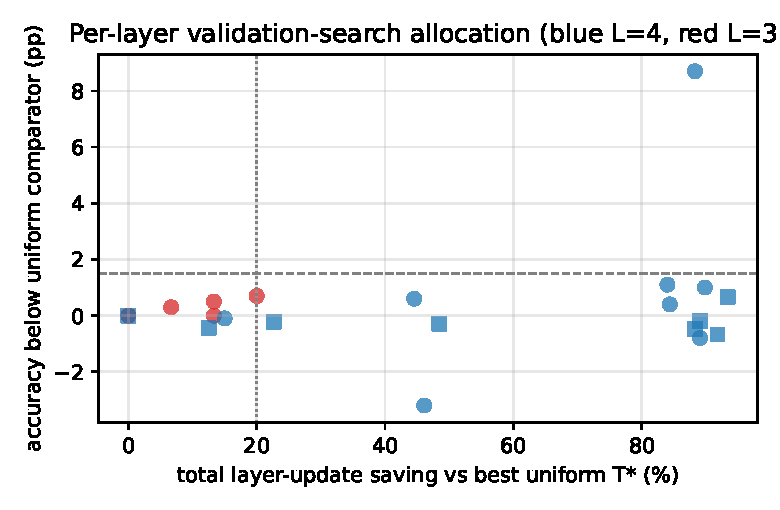
\includegraphics[width=0.92\columnwidth]{figures/fig8_allocation_regime.pdf}
\caption{Validation-searched per-layer windows against the best uniform budget at band, pilot
and held-out cells; blue marks $L=4$, red marks $L=3$. Points below the dashed line stay inside
the accuracy band; points right of the dotted line save at least $20\%$ of total layer-updates.
The deep regime carries the headroom; the $L=3$ cells cluster at the origin.}
\label{fig:allocation}
\end{figure}

\subsection{Per-layer windows in the deep regime}
\label{sec:allocation}

Where uniform timesteps are held to the worst layer's budget, per-layer windows have room to
work, and a validation search finds it. For each model we ran a coordinate descent over per-hidden-
layer windows $\{1,2,3,4,6,8,12,16\}$, maximising \emph{validation} accuracy at fixed
total-update budget (two rounds; the search never sees test labels), then evaluated the chosen
allocation once. Against the best uniform budget at band, the search preserves accuracy with
$22.7$--$93.4\%$ fewer total layer-updates on six of eight held-out $L=4$ configurations
(chameleon $2/4$, squirrel $4/4$), and on six of eight pilot $L=4$ cells ($44$--$90\%$); a random
allocation under the same search budget is worse or equal on the majority of cells. The mechanism
is visible in the numbers: at $L=4$ the uniform requirement explodes (the smallest uniform $T$
at band reaches the search cap on most cells) because the depth law holds every layer to the worst
layer's budget, and the search releases the low-gain layers from it.

The capability has a boundary, and the boundary is the result. On $L=3$ configurations the
uniform budget is already compact ($T^{*} \le 16$) and the same search finds almost nothing to
release ($1/8$ cells); the pre-registered mixed-$L$ screen (which required the effect on two thirds
of $16$ mixed cells) was not met ($37.5\%$), and the validated claim is therefore the deep-regime
one, confirmed at $L=4$ only. The idea family is prior art --- per-layer timesteps in conversion
are established \citep{ramesh2025pascal,guo2026mixed}, and search-based per-layer budgets already
save $1.67$--$3.84\times$ synaptic updates in \citet{nallathambi2022ldsnn}; what is measured here
is where the headroom lives on graphs and that a validation-only search reaches it.

\begin{figure}[t]
\centering
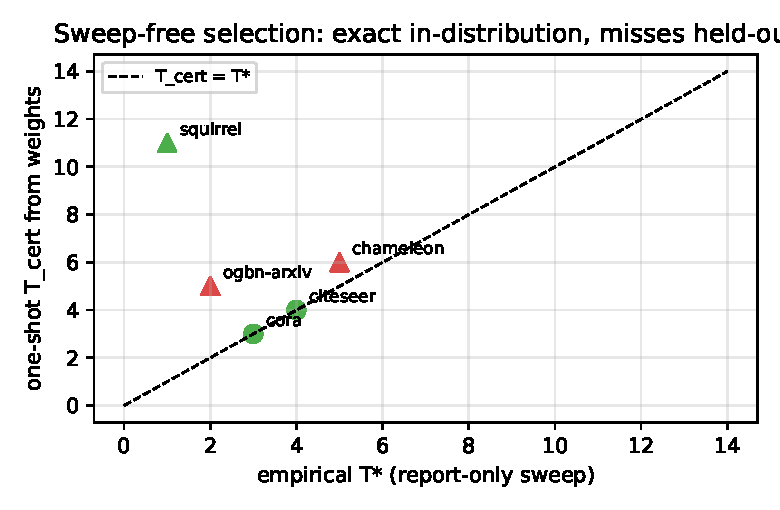
\includegraphics[width=0.92\columnwidth]{figures/fig9_transfer.pdf}
\caption{One-shot latency selection from weights: $T_{\mathrm{cert}}$ against the empirical
$T^{*}$, per graph. Green marks cells inside the accuracy band, red marks misses. The two
calibration graphs sit on the identity line; the held-out graphs do not.}
\label{fig:transfer}
\end{figure}

\subsection{What does not transfer across graphs}
\label{sec:transfer}

Three weight-derived routes were tried and each failed its pre-registered held-out gate, with a
measured failure mode each. (i) \emph{Closed-form window certificates}: the gain-equalised rule
starves low-gain layers to windows below four and loses $2$--$5.6$ points there; the two
certificate-based repairs (a margin floor, a per-layer sufficiency bound) over-provision to the
search cap on every cell --- the worst-case bound is $3.2$--$6.7\times$ conservative, exactly as
\secref{sec:theory} measures. The regime map is the residue: windows of four or more hold the band
at $8$--$29\%$ saving on $3/8$ pilot cells. (ii) \emph{Sweep-free latency selection}: a certificate
$T_{\mathrm{cert}}$ calibrated on two graphs is exact on those two ($\kappa = 1.0$, and a shuffled
calibration control is strictly worse) yet fails to transfer --- band hits on one of three held-out
graphs and $\kappa \in \{1.2, 11.0, 2.5\}$ --- under-provision on chameleon, $11\times$
over-provision on squirrel, and both failure modes together on arxiv. (iii) \emph{Gap prediction}
ranks models almost perfectly yet misses
the level by $4.6$ points. Within a configuration the identity is exact; the per-graph margin and
activation scales that the certificates need are not transferable across the
homophily/heterophily divide. The negative map is why the constructive result of
\secref{sec:allocation} is stated as a procedure with a validation sweep and not as a formula.

\section{Discussion}
\label{sec:discussion}

\subsection{Misalignment is a variance phenomenon, not a bias phenomenon}
\label{sec:variance}

It is tempting to describe the graph conversion error as ``noise from asynchronous arrival'' and to
expect more timesteps to wash it out. \eqnref{eq:split} says something sharper, and the measurements
agree. The error splits into a systematic part, which is a \emph{bias} with a closed-form correction,
and a zero-mean part whose magnitude is controlled not by the number of neighbours but by $\anorm$:
the neighbourhood converts a sum of worst-case deviations into a variance sum, so adding neighbours
helps rather than hurts. The diagnostic that separates the two is the share of the certificate each
term consumes. Without the bias, the systematic term is $26.1\%$, $24.5\%$ and $21.3\%$ of the bound
on Cora, CiteSeer and PubMed at $T=8$; with $\betastar$ it falls to $1.4\%$, $1.0\%$ and $0.7\%$. The
bias does not shrink the fluctuation at all---its half-width is $1/(2T)$ either way---which is
precisely why its benefit is concentrated at small $T$ and has vanished by $T=16$, and why an
experiment that only reported accuracy at large $T$ would conclude, wrongly, that the bias does
nothing.

The same decomposition explains an asymmetry that would otherwise look like a quirk. Sum aggregation
has row sums up to $169$ and, under a naive reading of \eqnref{eq:split}, should suffer a systematic
error two orders of magnitude larger than mean aggregation. It does not: the margin $\Deltan$ is
computed from the \emph{same} aggregated logits, so the relative error is $\rho$-invariant, and what
actually governs the conversion is $\anorm\lVert DW\rVert_{2}/(T\Deltan)$. We originally predicted
the opposite and were corrected by the experiment (\secref{sec:generality}); we report the
prediction, the refutation and the corrected account because the episode is the clearest evidence we
have that the identity, and not the intuition, is doing the work.

\subsection{How tight is the guarantee, and where is the slack}
\label{sec:tight}

A sufficient condition that certifies $68\%$ of nodes when $96\%$ are in fact correct invites the
question of whether the bound is merely loose or structurally loose. It is structurally loose, and
the slack has one address. Decomposing the bound per node (\secref{sec:theory}) shows that
$73$--$99\%$ of it is the Hoeffding term; the median ratio of bound to realised error is
$3.2$--$6.7\times$ for $T \ge 4$ (up to $8.4\times$ at $T=1$), and the Hoeffding half-width alone is
$1.3$--$2.3\times$ the realised 95th percentile of the fluctuation over the FTBC-configuration
subset ($1.3$--$4.1\times$ over all cells). The reason is a mismatch of
regimes: Hoeffding treats the $(m,h)$ sum as adversarial, using the worst-case half-width
$w = 1/(2T)$ for every term, whereas the residuals are close to uniform and independent, so the
realised sum concentrates like a variance sum. Replacing Hoeffding by a Bernstein bound---which uses
the residual variance we already measure---should tighten the constant by roughly $\sqrt{12}$, a
factor of $3.5$. We have not done this, because the theorem's job here is to identify \emph{which}
quantity sets the required latency ($\anorm\lVert DW\rVert_{2}/\Deltan$) and to certify without free
parameters; a tighter constant would raise the certificate's coverage without changing its message.
What matters for soundness is the other direction, and there the evidence is clean: the node-level
violation rate is $0.0$--$0.6\%$, comfortably inside the $\delta = 0.05$ budget, so the theorem is
never contradicted.

One honest limitation about the theorem's usefulness: it is not a recipe. $\Deltan$ is a property of
the trained model, so the statement cannot tell a practitioner in advance how many timesteps to
budget; it can only be evaluated after training. What it does give is the scaling and the ranking---why
the bias roughly halves the required $T$, why a graph with larger $\anorm$ needs more latency, and
why a conflict is decided by the margin rather than by the graph's size---and a diagnostic that a
practitioner can compute post hoc to see which nodes are at risk.

\subsection{Boundaries and threats to validity}
\label{sec:boundaries}

\paragraph{Operator.} The derivation needs a fixed, non-negative message-passing operator. Symmetric
GCN, mean and sum aggregation are covered; learned per-edge attention is not, unless the attention is
frozen into a fixed operator before conversion. This is a real restriction rather than a
technicality: an attention weight that changes per forward pass would break the very $\Ahat$ that
\eqnref{eq:identity} factorises.

\paragraph{Depth.} The recursion extends exactly to $L$ layers (\eqnref{eq:recursion}), and the
measured consequence is negative. The output error is amplified by the cumulative spectral gain $G=\prod_l\lVert M_l\rVert_{2}$, and the measured amplification follows $G^{0.95}$ with $r=0.990$ across nine cells (\secref{sec:depth}). At $L=4$ that is a $24$--$41\times$ amplification and a $21$-point deficit at $T=8$. Two natural repairs fail for a reason worth stating: gauge-normalising each layer is free for the ANN because ReLU is positively homogeneous, but the spike threshold is an absolute scale, so the renormalised network either falls silent or is bit-identical to the original once $\theta$ is rescaled with it. Computing $G$ before converting a backbone therefore tells the
practitioner whether the conversion is worth attempting.

\paragraph{The prediction that did not hold.} We set out to predict absolute accuracy from the weights and could not: the level is off by $4.6$ points even though the ordering is right. Two things are worth saying about that. The failure is not a tuning failure --- the model linearises around the margin, and in the cells where it errs the conversion has already destroyed most of the accuracy, so the linearisation is invalid rather than imprecise. And the ablation the mechanism implies does not fire: scrambling the per-node error scales, which should destroy the spatial correspondence that \eqnref{eq:sigma} predicts, leaves the error slightly \emph{better}. We therefore claim the ranking and not the level, and a reader who needs the absolute number should evaluate the closed form of \secref{sec:closed} instead, which is exact at two layers and costs one matmul.

\paragraph{Comparison scope.} The external arms in \tabref{tab:pareto} are
re-implementations of published formulations rather than reproductions of released
checkpoints; no released checkpoints exist for the rate-coded formulation at our splits.
\secref{sec:audit} reports the two codebase-level measurements that anchor the comparison,
and a companion paper \citep{companion} reports the full audit of the three pipelines that
publish code. We do not enter the large-scale benchmark of \citet{zhang2025sgnnbench},
which compares trained spiking GNNs at sizes where our conversion has not been validated.

\paragraph{Threshold regime.} \secref{sec:lemma1} assumes activations in $[0,\theta]$. With
$\theta = 1$ and no global rescaling the violating mass is at most about $1\%$ on the graphs we test,
and those units are carried by an explicit saturation term rather than ignored. At larger activation
scales the standard per-layer rescaling becomes necessary, and the theory then acquires an extra
factor of the inverse scale. We did not test that regime.

\paragraph{Scale.} The $169$k-node experiment asks whether conversion preserves its own ANN, and the
answer is yes. It does \emph{not} establish that our ANN is competitive on ogbn-arxiv; our
$169$k-node GCN is weaker than the best published models there, and widening it did not close the gap
within the budget we allowed. Any reading of that row as a state-of-the-art claim would be a
misreading, and \secref{sec:scale} is worded to prevent it.

\paragraph{Baselines.} Our strongest competitors are re-implementations of published
\emph{formulations}---direct training with a constant analogue input, and rate-coded direct
training---trained by us under our splits and seed budget. We did not reproduce any published
codebase, so we claim nothing about beating a specific published number. The compensating strength is
control: same architecture, same optimiser, same early stopping, same seeds. We also report two
dropout protocols for the direct baseline because they differ measurably, and the stronger one is the
one our claims are measured against.

\paragraph{Efficiency.} Spike counts and timesteps are proxies. They ignore membrane-update cost, memory access patterns and event-routing overhead, all of which matter on real hardware, and we never convert them into joules. We also tested whether the count can be bought down: pruning half the hidden units by activation mass cuts spikes by $23$--$36\%$ for at most $0.5$ points, and reaching a $40\%$ cut needs three quarters of the units and costs about one point. We report this as a trade-off, not as an energy win, and the gate we set for ourselves (spikes down $40\%$ at no more than $0.3$ points) fails on all three graphs.

\paragraph{One assumption is checked, not proven.} Uniformity of the sub-threshold residuals holds to
within $1\%$ on our graphs, and we report the check per run. It is an assumption about the activation
distribution of a trained network, and a network trained into strongly correlated activations could
violate it.

\subsection{Outlook}
\label{sec:outlook}

Two directions follow directly. The first is dynamic graphs: ``train once, deploy at any latency'' is
worth most when the latency budget changes at inference time, which is the normal situation in
streaming settings, and conversion is the only route offering it. The second is to freeze
attention---convert a trained attention model by materialising its attention into a fixed operator
and bounding the resulting perturbation---which would extend the formulation from fixed aggregators
to the attention family without abandoning the exact identity. Beyond the method, the exercise
suggests that the non-vision frontier of conversion needs its own analyses rather than transplanted
recipes: the two things vision conversion takes for granted, a row-stochastic operator and a decoder
that can afford to count, both fail here, and each failure produced a design change rather than a
numerical nuisance.

The negative map of \secref{sec:transfer} deserves its own reading. The identity and the laws are
\emph{in-configuration} statements: they characterise a trained model and its conversion exactly.
The moment a decision must be made for a \emph{new} graph from weights alone --- how many timesteps,
how to split them across layers --- the certificates need per-graph margin and activation scales
whose transfer we could not establish by any of three routes. We offer this as an open problem with
measured failure modes rather than as a limitation paragraph: the practical guidance is to run a
small validation search (\secref{sec:allocation}) and to treat weight-only certificates as
hypotheses about a new graph until they are recalibrated there.

The accounting sensitivity of \secref{sec:accounting} is a methodological hazard for the
literature this paper sits in. A converted network and a linear-readout external arm exchange the
``cheaper'' label when the unit changes from static synaptic updates to spike events, and a
reference implementation can carry a cost model for a layer its code never trains. Comparisons of
SNN efficiency on graphs should therefore state the counting convention, ship the accounting, and
treat the ranking as convention-conditional --- the same discipline the identity enforces on the
accuracy side.

\section{Conclusion}
\label{sec:conclusion}

We formulated ANN-to-SNN conversion for graph node classification and found that the graph-specific
obstruction has a name and an algebra. Neighbours fire at different times, so the second layer
integrates a locally reordered pre-activation; writing that down yields an exact error identity, and
the identity yields four things in turn: a closed-form forward bias $\betastar = \theta/(2T)$ that
removes the systematic part of the error and makes the method parameter-free; a membrane readout
that removes the output quantisation and clipping that counting imposes, and that we prove---and
verify to four decimals---is exactly invariant to the order of upstream spikes, which the count
decoder is not; a margin-recovery theorem whose required latency depends on neighbourhood geometry
rather than on graph size; and, once the identity is extended to $L$ layers, a depth law: the error
is amplified by the cumulative spectral gain $G=\prod_l\lVert M_l\rVert_2$ of the trained ANN, and
the amplification follows $G^{0.95}$ with $r=0.990$ over nine cells, so what a deep model will cost
in latency is computable from its weights before any simulation.

At seven seeds across six graphs, converted networks reach their ANN to within $1.5$ points at
$T \le 8$, and on a protocol shared by four arms they are never dominated: at matched accuracy they
cost $2$--$23\times$ fewer synaptic operations than a trained spiking network on two of three graphs
under the static-update accounting --- the ordering is convention-conditional
(\secref{sec:accounting}), which is itself one of the paper's findings --- and on CiteSeer they are
the only arm that reaches the band at all. The identity also buys a concrete decision: in the deep
regime, where uniform budgets explode with the depth law, a validation-only per-layer window search
keeps the accuracy band with $22.7$--$93.4\%$ fewer layer-updates on six of eight held-out
four-layer cells (\secref{sec:allocation}), while the weight-only routes fail to transfer
(\secref{sec:transfer}). External anchors frame, and do not enter, this protocol: SpikeGraphormer's
released pipeline reaches $74.0$ on Cora below the conversion at $T=16$, and SpikeGCL's
self-supervised pipeline reaches $86.6$ above every arm here. The converted networks train one
model instead of five, and they degrade in the way the theory predicts when the aggregation
operator, the threshold, the width or the decoder is changed.

The limits are as informative as the results. Conversion does not
buy energy: at matched accuracy it emits more spikes than a trained spiking network, and pruning
half the hidden units recovers only a third of the excess at a fraction of a point of accuracy.
Depth is not bought either: the amplification cannot be reparametrised away, because the spike
threshold is an absolute scale while the ReLU that would let one rescale it is homogeneous---and at
$L\ge3$ the closed form that makes the two-layer case free of simulation breaks too, for the same
reason, the reset. The count decoder does not free the computation from temporal ordering, since
only the membrane decoder has that. And averaging over the threshold and the initial
potential---axes that cost no spikes---never beats the ANN, whereas nine independently trained ANNs
beat it by about a point on every graph, so what helps is ensembling models and not re-sampling one
model's discretisation error. The published numbers cannot be used as baselines without checking:
the two anchors we could place beside our own, measured from their authors' code on the public
split, bracket the conversion rather than rank it.

A prediction that failed is reported alongside them. The laws rank candidate models almost
perfectly ($\rho=0.967$) but miss the absolute conversion gap by $4.6$ points, and the ablation that
would have confirmed the mechanism does not. What survives is narrower and more useful
than a transferable predictor: conversion is a statement about how a computation is discretised,
on a graph the discretisation happens along the neighbourhood as well as along time, and the two
quantities that decide whether a given model converts well---its activation mass and its cumulative
spectral gain---can both be read off the trained weights before a single spike is simulated.


\bibliographystyle{plainnat}
\bibliography{refs}

\end{document}
